%% Template para dissertação/tese na classe UFBAthesis
%% versão 1.0
%% (c) 2005 Paulo G. S. Fonseca
%% (c) 2012 Antonio Terceiro
%% (c) 2014 Christina von Flach
%% www.dcc.ufba.br/~flach/ufbathesis

%% Carrega a classe ufbathesis
%% Opções: * Idiomas
%%           pt   - português (padrão)
%%           en   - inglês
%%         * Tipo do Texto
%%           bsc  - para monografias de graduação
%%           msc  - para dissertações de mestrado (padrão)
%%           qual - exame de qualificação de mestrado
%%           prop - exame de qualificação de doutorado
%%           phd  - para teses de doutorado
%%         * Um­dia
%%           scr  - para verão eletrônica (PDF) / consulte o guia do usuário
%%         * Estilo
%%           classic - estilo original a la TAOCP (deprecated)
%%           std     - novo estilo a la CUP (padrão)
%%         * Paginação
%%           oneside - para impressão em face única
%%           twoside - para impressão em frente e verso (padrão)
\documentclass[bsc, classic, a4paper, oneside]{ufbathesis}
\DeclareMathAlphabet      {\mathbfit}{OML}{cmm}{b}{it}

%% Preambulo:
\usepackage{xcolor} 
%% This control colors of equations, tables, figures, links, references and etc.
\hypersetup{
  colorlinks,
  linkcolor={red!30!black},
  citecolor={blue!50!black},
  urlcolor={blue!50!black}
  %linkcolor={black},
  %citecolor={black},
  %urlcolor={black}
}
\usepackage[utf8]{inputenc}
\usepackage{graphicx,url}
\usepackage{caption}
\usepackage{lipsum}
\usepackage{amsmath}
\usepackage{mathtools}
\usepackage{enumitem}
\graphicspath{{assets/}}
\usepackage{algorithm2e}
\usepackage{qtree}
\usepackage{amstext} % Useful package to put accents in mathmode with \text
\usepackage{multirow}
\usepackage{array,booktabs}
%\everymath=\expandafter{\the\everymath\displaystyle}
\everymath{\displaystyle}
\SetKwRepeat{Do}{faça}{enquanto} % Macro to allow do while in algorithm2e
\SetKwBlock{Begin}{início}{fim}
\SetKwFor{For}{para}{faça}{fim} 
\SetKwFor{ForEach}{para cada}{faça}{fim} 
\SetAlgorithmName{Algoritmo}{Lista de Algoritmos}

% ---
% Citacao direta com mais de 3 linhas - ABNT NBR 10520/2002 - 5.3
\newlength{\ABNTEXcitacaorecuo}% recuo de 4 cm da margem esquerda
\setlength{\ABNTEXcitacaorecuo}{4cm}
\newcommand{\ABNTEXfontereduzida}{\footnotesize}
\newenvironment*{citacao}[1][default]
{
  \list{}%
  \ABNTEXfontereduzida%
  \addtolength{\leftskip}{\ABNTEXcitacaorecuo}%
  \item[]%
  %\begin{SingleSpace}%
  %\ifthenelse{\not\equal{#1}{default}}{\itshape\selectlanguage{#1}}{}%
}
{ 
  %\end{SingleSpace}%
  \endlist%
}

% Universidade
\university{UNIVERSIDADE FEDERAL DA BAHIA}

% Endereço (cidade)
\address{Salvador}

% Instituto ou Centro Acadêmico
\institute{INSTITUTO DE MATEMÁTICA}

% Nome da biblioteca - usado na ficha catalográfica
\library{BIBLIOTECA REITOR MAC\^{E}DO COSTA}

% Programa de pós-graduação
\program{Programa de Graduação em Ciência da Computação}

% Area de titulação
\majorfield{CI\^{E}NCIA DA COMPUTA\c{C}\~{A}O}

% Titulo da dissertação
\title{Detecção inteligente de efeitos colaterais indesejáveis na Internet das coisas - um estudo de caso no Home Network System}

% Data da defesa
% e.g. \date{19 de fevereiro de 2003}
\date{31 de outubro de 2016}

% Autor
% e.g. \author{Jose da Silva}
\author{Heron Sanches Gonçalves Pires Ferreira}

% Orientador(a)
% Opção: [f] - para orientador do sexo feminino
% e.g. \adviser[f]{Profa. Dra. Maria Santos}
\adviser[f]{Profa. Dra. Daniela Barreiro Claro}

% Orientador(a)
% Opção: [f] - para orientador do sexo feminino
% e.g. \coadviser{Prof. Dr. Pedro Pedreira}
% Comente se não se aplicar
%\coadviser{NOME DO(DA) CO-ORIENTADOR(A)}

%% Inicio do documento
\begin{document}

\pgcompfrontpage{}

%% Parte pre-textual
\frontmatter

\pgcomppresentationpage

% Ficha catalográfica
\authorcitationname{Ferreira, Heron Sanches Gonçalves Pires} % e.g. Terceiro, Antonio Soares de Azevedo
\advisercitationname{Claro, Daniela Barreiro} % e.g. Chavez, Christina von Flach Garcia
\catalogtype{Monografia (Graduação)} % e.g. ``Tese (Doutorado)''
\catalogtopics{``1. Efeitos Colaterais. 2. Internet das Coisas. 3. Home Network System. 4.
  Serviço WEB. 5.Dispositivos. 6.REST. 7.Rede Neural. 8.Multilayer Perceptron''} 
\catalogcdd{CDD 005.13307} % e.g. ``CDD 20.ed. XXX.YY'' (esse número vai lhe ser dado pela biblioteca)
\catalogingsheet

% Termo de aprovação
\approvalsheet{Salvador, 31 de outubro de 2016}{
   \comittemember{Profa. Dra. Daniela Barreiro Claro}{Universidade Federal da Bahia}
   \comittemember{Prof. Dr. Cássio Vinicius Serafim Prazeres}{Universidade Federal da Bahia}
   \comittemember{Prof. Dr. }{Universidade Federal da Bahia}
}

% Dedicatória
% Comente para ocultar
\begin{dedicatory}
  ... //TODO
\end{dedicatory}

% Agradecimentos
\acknowledgements
Obrigado minha mãe, por sua dedicação durante todos estes anos. Obrigado minha tia Suzi, por ter me dado oportunidade de estudo e sempre está disposta a me ajudar em qualquer situação. Obrigado as forças boas que vêem me guiando e me ajudando. Obrigado Daniela e Roberto pela orientação prestada para este trabalho.


% Epigrafe
%  \begin{epigraph}[Tarde, 1919]{Olavo Bilac}
%  Ultima flor do Lácio, inculta e bela,\\
%  Es, a um tempo, esplendor e sepultura;\\
%  Ouro nativo, que, na ganga impura,\\
%  A bruta mina entre os cascalhos vela.
%  \end{epigraph}
\begin{epigraph}[1687]{Isaac Newton}
  O que sabemos é uma gota, o que ignoramos é um oceano.
\end{epigraph}

% Resumo em Português
\resumo
Diversos dispositivos têm sido incorporados em ambientes domésticos através dos \textit{Home Server} (HS) com o intuito de automatizar as tarefas cotidianas de uma casa inteligente. Estes dispositivos podem ser disponibilizados como serviços Web RESTFul. Porém, muitos destes dispositivos independentes não conseguem atender aos requisitos dos usuários. Assim, há a necessidade de composição destes com outros dispositivos para prover funcionalidades que atendam a esses requisitos. Quando existe uma composição de dispositivos, o comportamento de pelo menos um destes pode provocar interação de características com efeitos colaterais indesejáveis. Assim, o presente trabalho propõe detectar efeitos colaterais indesejáveis entre dispositivos utilizando-se do \textit{ensemble} DECORATE. Para isto, observou-se o comportamento físico e as mensagens trocadas entre os dispositivos. Através do conjunto de dados obtidos realizou-se um processo classificatório e implantou um classificador no FIM (\textit{Feature Interaction Manager}) do HS, mostrando que é possı́vel detectar efeitos colaterais indesejáveis entre dispositivos.

% Palavras-chave do resumo em Português
\begin{keywords}
TODO
\end{keywords}

% Resumo em Ingles
\abstract
Many devices have been put on domestics environments through the Home Servers with the aim of automate the daily tasks of a smart home. But, some devices when alone do not attend the user specifications. Then, there is the needed to compose them to provide features that are accord to them specifications. When there is a device's composition, the behave of at least one of them can cause feature interactions with undesirable side effects. So, this work proposes detect undesirable side effects between devices using the ensemble DECORATE. For it propose was realized observations of the physical devices behave and the messages changed by these devices, which were made available how Web RESTFul services. Through the data collected was made a classification process and as the final result was obtained a model with more than 90\% of precision. It was put into FIM (Feature Interaction Manager) of the Home Network System (HNS), showing that is possible detect undesirable side effect between these devices.

% Palavras-chave do resumo em Ingles
\begin{keywords}
TODO
\end{keywords}

% Sumario / Índice
% Comente para ocultar
\tableofcontents

% Lista de figuras
% Comente para ocultar
\listoffigures

% Lista de tabelas
% Comente para ocultar
\listoftables

\renewcommand*{\listalgorithmcfname}{Lista de algoritmos}
\listofalgorithms
\addtocontents{loa}{\def\string\figurename{Algoritmo}}

%% Parte textual
\mainmatter

% Eh aconselhável criar cada capitulo em um arquivo separado, digamos
% "capitulo1.tex", "capitulo2.tex", ... "capituloN.tex" e depois
% inclui-los com:
% \include{capitulo1}
% \include{capitulo2}
% ...
% \include{capituloN}
%
% Importante: Use \xchapter ao invés de \chapter, se quiser colocar texto antes do inicio do capitulo.

\xchapter{Introdução}{Uma breve introdução sobre do que se trata esta monografia e a maneira como o texto está organizado.}
\label{ch:intro}

A Internet nesta última década tem contribuído de forma significativa na economia e sociedade, deixando como legado uma sólida infraestrutura de rede de comunicação. O seu maior disseminador nesse período vem sendo \textit{World Wide Web}(WWW), o qual permite o compartilhamento de informação e mídia de forma global \cite{Chandrakanth:2014}.

A Internet está se tornando cada vez mais presente no cotidiano, devido, por exemplo, ao crescente número de usuários de dispositivos móveis, os quais possuem tecnologias de conexão com a Internet, as quais cada dia tornam-se mais acessíveis \cite{Chandrakanth:2014}.

Em 2010 havia aproximadamente 1,5 bilhão de PCs conectados à Internet e mais que 1 bilhão de telefones móveis \cite{Sundmaeker:2010}. Segundo Gartner\footnotemark \footnotetext{\url{http://www.gartner.com/newsroom/id/3165317}}, 6,4 bilhões de coisas estarão conectadas até o final de 2016 e, de acordo com estimativas da CISCO\footnotemark \footnotetext{\url{http://www.cisco.com/c/en/us/solutions/collateral/enterprise/cisco-on-cisco/Cisco_IT_Trends_IoE_Is_the_New_Economy.html}}, em 2020 esse número atingirá cerca de 50 bilhões. A previsão de \cite{Sundmaeker:2010}, a qual dizia que a denominada Internet dos PCs seria movida para o que se chama de Internet das Coisas fica então mais evidente neste atual cenário.

\textit{Internet of Things} (IoT), traduzido para o português como Internet das Coisas, pode ser definida como uma rede de coisas que têm a capacidade de sentir, identificar e compreender o ambiente em que estão imersas \cite{Ashton:2009}. ``Coisas ou objetos'', tais como, RFID tags, sensores, telefones móveis, dentre outros, através de esquemas de endereçamento único são capazes de interagir com os outros e cooperar com seus vizinhos para alcançar um objetivo em comum \cite{Atzori:2010}.

Uma definição tecnológica para IoT pode ser como em \cite{Sundmaeker:2010}, o qual diz que IoT é parte integrante da futura Internet e pode ser definida como uma infraestrutura de rede global dinâmica com capacidades de autoconfiguração baseada nos padrões e interoperabilidade dos protocolos de comunicação onde coisas físicas e virtuais têm identidade, atributos físicos, personalidade virtual, usam interfaces inteligentes e, são integradas dentro da rede de informações.

Apesar da grande potencialidade da Internet das Coisas, a qual gerou em 2015 um faturamento em torno de 130,33 bilhões de dólares americanos e tem prospecção de chegar até 883.55 bilhões em 2020\footnotemark \footnotetext{http://www.marketsandmarkets.com/Market-Reports/iot-application-technology-market-258239167.html}, ainda existem muitos desafios a serem vencidos, tais como segurança da informação \cite{Roman:2013}, armazenamento e processamento de grande quantidade de dados \cite{Zaslavsky:2013}, dentre outros. Adentrando em um dos dessafios da IoT, o da disponibilidade de uma interface de comunicação e programação comum aos objetos, pode-se disponibilizar os dispositivos como serviços Web RESTFull, desta forma pode-se utilizar os protocolos Web como linguagem comum de integração dos dispositivos à Internet \cite{Franca:2011, Mineraud:2016}.

Diante deste cenário onde diversos dispositivos são combinados para alcançar um objetivo em comum \cite{Kranz:2010, Atzori:2010, Whitmore:2015}, e da crescente adição destes à IoT, surge a necessidade de tratar um outro problema ainda não citado, que ocorre quando a composição de dispositivos (os quais oferecem alguma funcionalidade) leva a um comportamento não esperado (interação de características) por esta composição, o qual pode resultar em um estado inconsistente, instabilidade ou dados imprecisos - efeito colateral indesejável \cite{NHLABATSI:2008}.

**falar de algumas posíveis causas**

**falr tudo o que o trabalho propoe**
Assim, o presente trabalho propõe detectar efeitos colaterais indesejáveis entre dispositivos através da meta-classificação, metodologia que utiliza um conjunto de classificadores para construir diversas hipóteses (modelos). Então, é utilizado o conhecimento de cada modelo afim de se chegar em uma decisão final mais confiável \cite{Melville:2004}.

Os dados de treino foram gerados manualmente a partir de um conjunto de objetos do cenário ``Levar compras'', o qual foi utilizado no estudo de caso do \textit{Home Network System}.

Os resultados obtidos demonstraram que através da meta-classificação foi possível detectar os efeitos colaterais indesejáveis com mais de 90\% de precisão.

O restante deste trabalho está organizado da seguinte maneira:

\begin{itemize}
\item Capítulo \ref{ch:theory}: Apresenta todo embasamento teórico necessário para compreender o estudo realizado neste trabalho.
\item Capítulo \ref{ch:proposta}: Esse capítulo descreve a proposta para detecção de efeitos colaterais indesejáveis no cenário ``Levar compras''.
\item Capítulo \ref{ch:validacao}: Trata dos procedimentos realizados para validar a proposta de pesquisa deste TCC.
\item Capítulo \ref{ch:conclusion}: Este capítulo é uma síntese da investigação e dos experimentos realizados neste TCC.
\end{itemize}


\xchapter{Fundamentação Teórica}{Este capítulo tem como objetivo fundamentar as bases necessárias dos campos de estudos utilizados nesta monografia.}
\label{ch:theory}

\section{Internet das coisas}
\label{sec:iot}
A Internet nesta última década tem contribuído de forma significativa na economia e sociedade, deixando como legado uma notável infraestrutura de rede de comunicação. O seu maior disseminador nesse período vem sendo \textit{World Wide Web}(WWW), o qual permite o compartilhamento de informação e mídia de forma global\cite{Chandrakanth:2014}.

No âmbito da economia, por exemplo, o E-Commerce permitiu potencializar as vendas de produtos e serviços, com um faturamento estimado para o ano de 2016 de aproximadamente 56,8 bilhões de reais no Brasil, segundo ecommercenews\footnotemark \footnotetext{https://ecommercenews.com.br/noticias/pesquisas-noticias/e-commerce-brasileiro-deve-crescer-18-e-faturar-r-568-bilhoes-em-2016}. Além do benefício direto para sociedade provindo do E-Commerce, onde as pessoas podem realizar pesquisa de preços de serviços e produtos e, adquiri-los de forma cômoda, sem precisar se deslocar até um ponto de venda, a Internet dispõe para a sociedade diversas outras oportunidades, como cursos a distância oferecidos por diversas universidades de todo o mundo, a exemplo dos cursos disponibilizados pela plataforma Coursera\footnotemark \footnotetext{\url{https://pt.coursera.org/}}. 

A Internet está se tornando cada vez mais persistente no cotidiano, devido, por exemplo, ao crescente número de usuários de dispositivos móveis, os quais possuem tecnologias de conexão com a Internet, as quais cada dia tornam-se mais acessíveis (presentes em locais que não tinham e, mais baratas)\cite{Chandrakanth:2014}.

Em 2010 havia aproximadamente 1,5 bilhão de PCs conectados a Internet e mais que 1 bilhão de telefones móveis\cite{Sundmaeker:2010}. Segundo Gartner\footnotemark \footnotetext{\url{http://www.gartner.com/newsroom/id/3165317}}, 6,4 bilhões de coisas estarão conectadas até o final de 2016 e, em 2020 esse número atingirá cerca de 20,8 bilhões. A previsão de \cite{Sundmaeker:2010}, a qual dizia que a denominada Internet dos PCs seria movida para o que se chama de Internet das Coisas fica então mais evidente neste atual cenário.

A ideia básica da \textit{Internet of things (IoT)}, traduzido para o português como Internet das Coisas é a presença pervasiva de uma variedade de "coisas ou objetos", tais como RFID tags, sensores, telefones móveis, dentre outros. Os quais, através de esquemas de endereçamento único são capazes de interagir com os outros e cooperar com seus vizinhos para alcançar um objetivo em comum\cite{Atzori:2010}. Outros exemplos de "coisas ou objetos" podem ser pessoas, geladeiras, televisores, veículos, roupas, medicações, livros, passaportes, contanto que possam ser identificadas unicamente e possam se comunicar com as outras coisas e/ou possam ser acessados remotamente por humanos.

Dentre as diversas definições de Iot pode-se citar duas, a primeira define de maneira mais geral, tanto a atual realidade, quanto a prospecção futura. Já a segunda especifica melhor como deve ser o cenário ideal da Internet das Coisas, pois já embuti explicitamente os conceitos de capacidades de autoconfiguração, interoperabilidade e interfaces inteligentes.
\begin{enumerate}
\item Segundo\cite{iot2020:2008}, \textit{Internet of Things} significa rede mundial de objetos unicamente endereçáveis e interconectados, seguindo os protocolos dos padrões de comunicação.
\item IoT é parte integrante da futura Internet e pode ser definida como uma infraestrutura de rede global dinâmica com capacidades de autoconfiguração baseada nos padrões e interoperabilidade dos protocolos de comunicação onde coisas físicas e virtuais têm identidade, atributos físicos, personalidade virtual, usam interfaces inteligentes e, são integradas dentro da rede de informações \cite{Sundmaeker:2010}.
\end{enumerate}

Diante deste cenário da IoT, pode-se citar exemplos de aplicações em diversos domínios, tais como, logística e transporte; cuidados com a saúde; ambiente inteligente (casa (seção \ref{sec:hns}), escritório);\cite{Atzori:2010} verificação de procedência alimentícia; dentre outros. Abaixo se tem uma breve descrição de duas aplicações, uma na área de cuidados com a saúde e outra na verificação de procedência de alimentos, respectivamente.

\begin{itemize}
\item Dispositivos implantáveis com capacidade de comunicação sem fio podem ser utilizados para armazenar registros sobre a saúde de um paciente em situações de risco e podem ser decisivos para salvar a vida do paciente. A capacidade de ter acesso a essas informações nessas circunstâncias fazem com que hospitais possam saber de imediato como tratar um paciente que esta a caminho. Esta possibilidade é especialmente útil para pessoas com diabetes, câncer, problemas de coração na artéria coronária, doenças do pulmão, assim como as pessoas com implantes médicos complexos, tais como, marcapassos, tubos, transplantes de órgãos e aqueles que podem ficar inconscientes e incapazes de comunicar-se durante uma operação. \cite{Weber:2010}
\item Rastreabilidade de produtos alimentícios ajudam os usuários a verificar a origem de um produto, assim como informações de composição química, dentre outros. Mas também previne de doenças não desejadas. Por exemplo, avisos atuais sobre a mercadoria em questão podem ser disponibilizados à medida que o produto sai da origem e vai passando para os outros níveis de consumo, desta forma os consumidores podem evitar o contágio de doenças como gripe aviária e, encefalopatia espongiforme bovina (EEB), mais conhecida como doença da vaca louca.\cite{Weber:2010}
\end{itemize}

Apesar da grande potencialidade da visão da Internet das Coisas, a qual gerou em 2015 um faturamento em torno de 130,33 bilhões de dólares americanos e tem prospecção de chegar até 883.55 bilhões em 2020\footnotemark \footnotetext{http://www.marketsandmarkets.com/Market-Reports/iot-application-technology-market-258239167.html}, ainda existem muitos desafios a serem vencidos, tais como segurança da informação, armazenamento e processamento de grande quantidade de dados, dentre outros. Adentrando um pouco em um dos desafios da IoT, o da disponibilidade de uma interface de comunicação (acesso aos serviços e informações dos dispositivos) e programação comum aos objetos, pode-se dizer que a falta desta padronização faz com que se torne oneroso o desenvolvimento de aplicações para o objeto, pois cada coisa possui suas próprias interfaces, logo para cada dispositivo um desenvolvimento a parte. Mais difícil ainda é prover uma única funcionalidade ou serviço com a composição dos diversos objetos. Para diminuir a dificuldade deste cenário, pode-se disponibilizar os dispositivos como serviços WEB (seção \ref{subsec:dispositivosWeb}), assim sendo se pode utilizar os protocolos WEB como linguagem comum de integração dos dispositivos a Internet.\cite{Franca:2011}

\subsection{Serviços Web}
\label{ws:webservices}
Segundo\cite{Dustdar:2005}, um serviço Web é um sistema identificado por uma URL\footnotemark \footnotetext{Acrônimo para Uniform Resource Locator e é uma referência (um endereço) para um recurso na Internet.\cite{oracle:url}}, no qual suas interfaces públicas são definidas e descritas usando XML\footnotemark \footnotetext{Extensible Markup Language (XML) é uma simples e flexível linguagem de marcação utilizada para codificar documentos através de regras produzidas por humanos, as quais podem ser manipulados (compreendidas) por máquinas \cite{w3c:xml}\cite{w3c:xmlschema}} e, suas definições podem ser descobertas por outros sistemas. Sistemas então podem interagir com os serviços Web utilizando suas definições e descrições. Através destas utiliza-se mensagens XML que são transmitidas seguindo os protocolos padrão (definidos por W3C\footnotemark \footnotetext{\url{https://www.w3.org/}}) da Internet para que haja tal interação.

Serviços Web surgiram tendo como principal foco o reúso de aplicações existentes (dentre as quais incluíam código fonte legado) para que pudessem se integrar de forma leve com outras aplicações, geralmente essa integração tinha como referência o desejo de  novas formas de compartilhamento dos serviços ao longo das diversas linhas do negócio ou entre parceiros. Para melhor entender o propósito dos serviços Web, considere, como exemplo, uma companhia de seguros que decidiu oferecer um serviço de cotação on-line. Então em vez de desenvolver toda a aplicação do início, a empresa utiliza-se do serviço Web de outra empresa (especializada em cálculos de seguro). Este serviço pode, por exemplo, oferecer um formulário de cotação e, após o cliente informar os dados necessários, o serviço Web apresentará uma cotação baseado nos dados informados. Além disso, caso o cliente escolher comprar tal seguro, pode-se ainda utilizar de outro serviço Web, oferecido por uma outra empresa, o qual processará o pagamento de acordo com os dados passados para ele e então retorna o resultado do processamento para o cliente e para a empresa original(que desejou construir o serviço de cotação on-line)\cite{Papazoglou:2008}. O cenário da Figura \ref{fig:ws_purchase_order} demonstra um outro exemplo de uso de diferentes serviços para prover um único serviço, o de um pedido de uma ou mais mercadorias, ambiente comum do E-Commerce.

\begin{figure}[!htb] \centering 
  \centering
  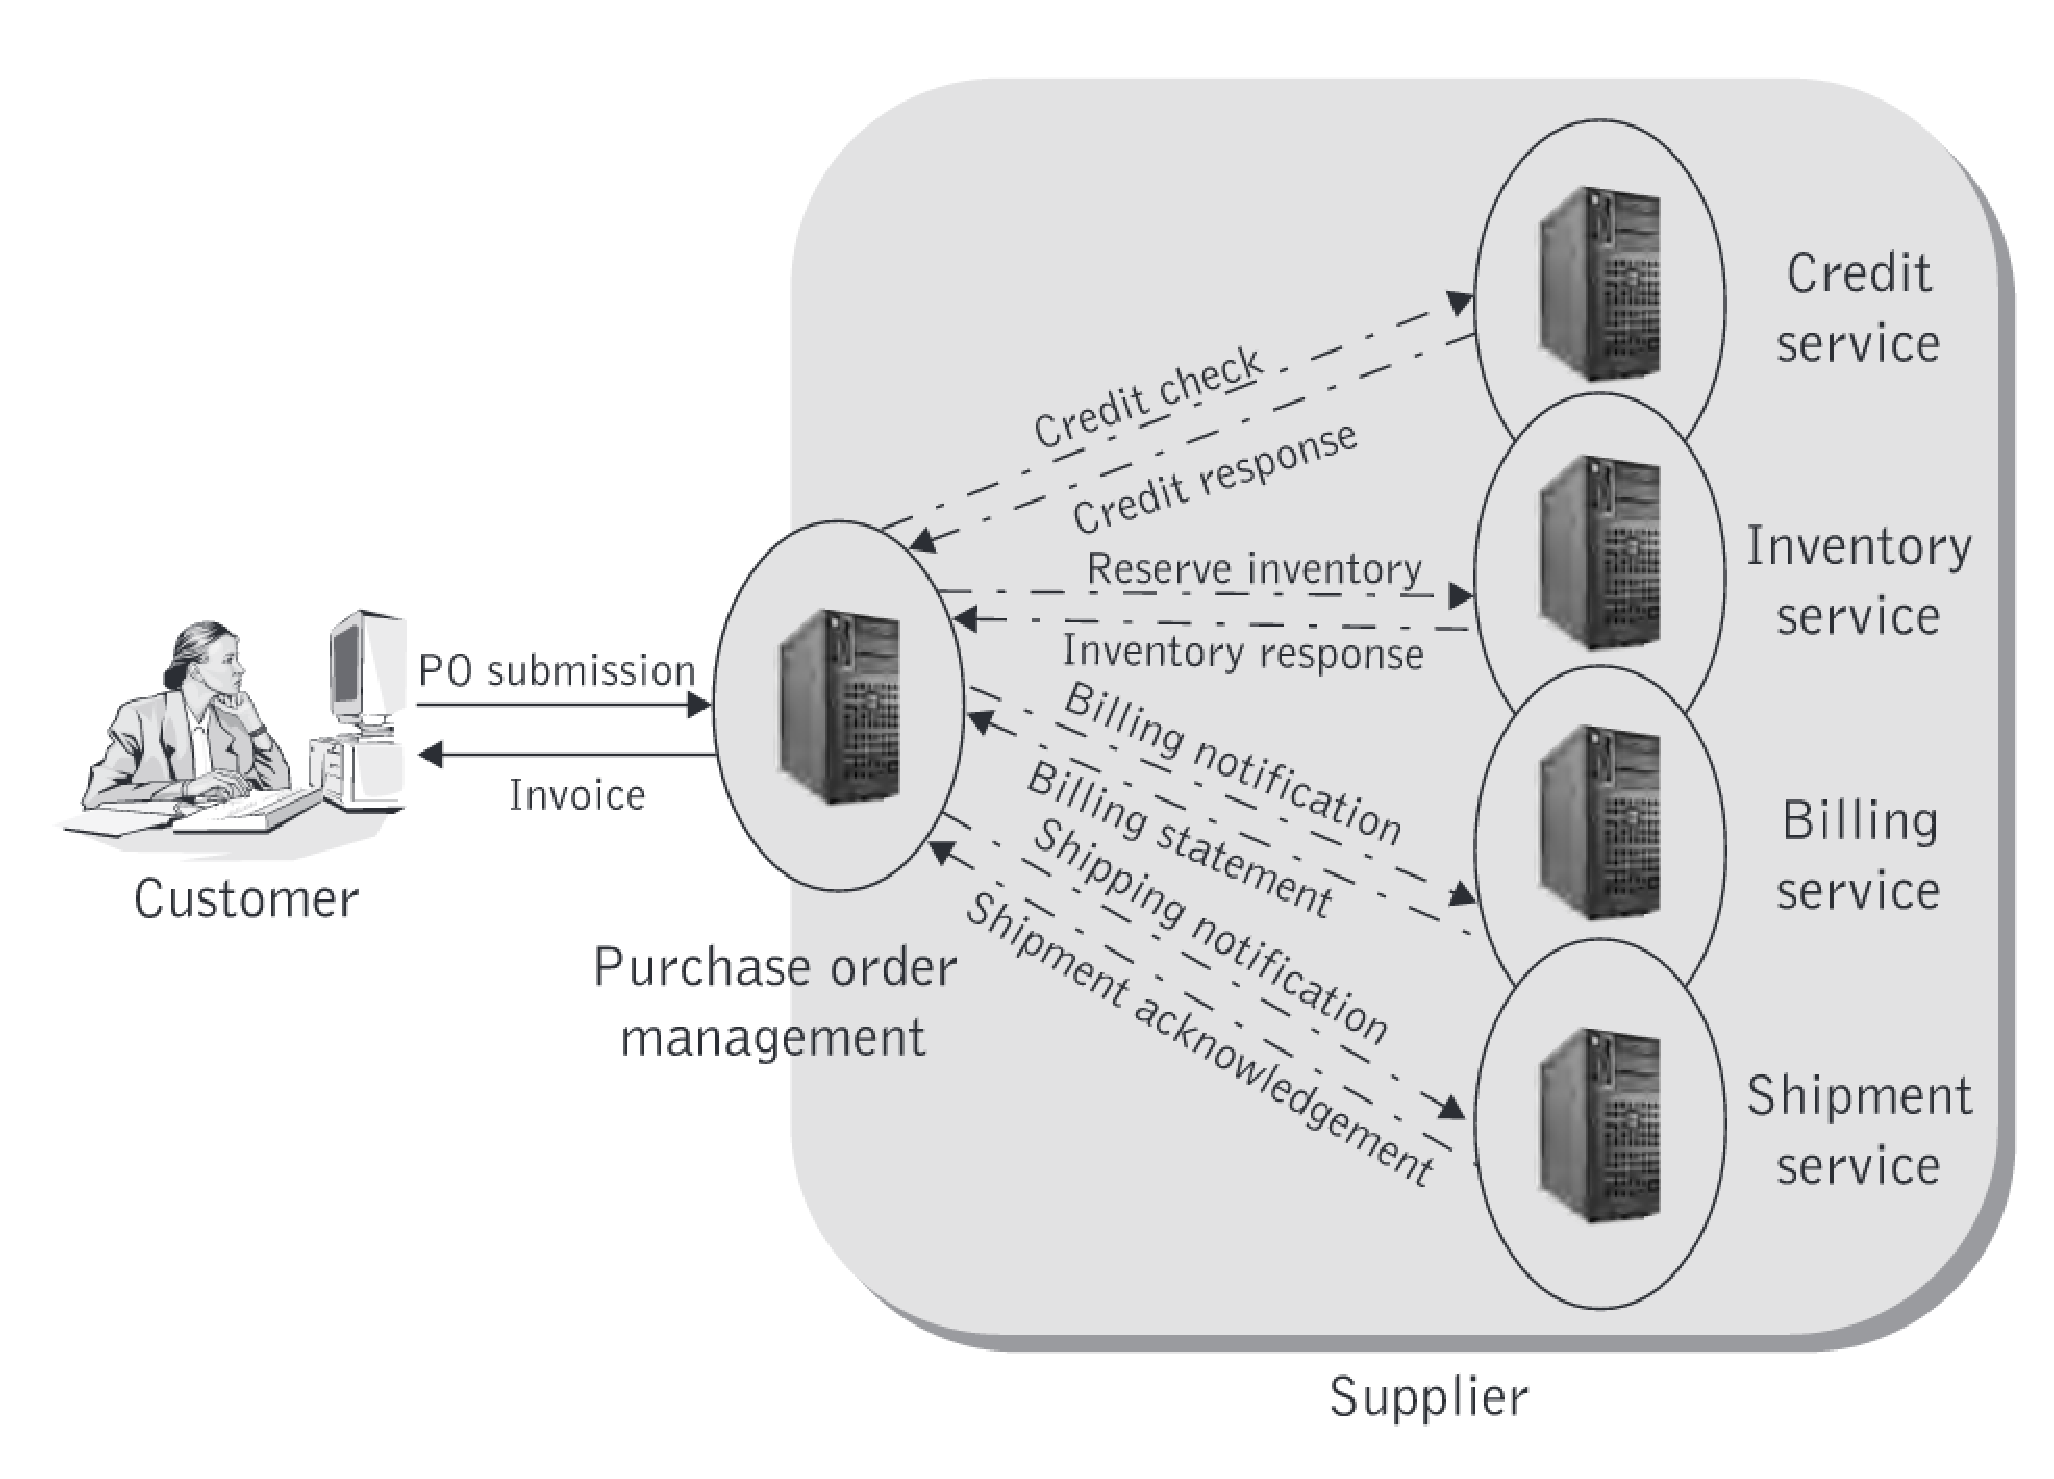
\includegraphics[width=0.8\columnwidth]{fundamentacao/webservice_purchase_order} 
  \caption{Utilização de diferentes serviços Web para prover o serviço de pedido de um E-Commerce.\cite{Papazoglou:2008}} 
  \label{fig:ws_purchase_order}
\end{figure}

O cenário do serviço(Figura \ref{fig:ws_purchase_order}) pode ser descrito da seguinte forma:
\begin{enumerate}
\item \textit{Consumer}(Consumidor) escolhe seu(s) produto(s), informa dados do cartão de crédito e outras informações necessárias e, clica no botão comprar. Requisição é enviada ao \textit{Purchase order management}(Gerenciador de pedidos de compra).
\item O gerenciador então verifica se o cartão do cliente tem crédito suficiente através da funcionalidade \textit{Credit check} do serviço \textit{Credit Service} e, o serviço dá uma resposta.
\item Gerenciador capta a resposta e, caso cliente tenha crédito suficiente, inicia o processo de reserva do pedido através da funcionalidade textit{Reserve inventory} do serviço \textit{Invetory service}.
\item Gerenciador capta resposta \textit{Inventory response}, caso o pedido tenha sido reservado com êxito, o gerenciador utiliza o \textit{Billing service} para processar o pagamento.
\item \textit{Billing service} retorna o estado do pagamento, se pagamento foi processado com êxito o gerenciador utiliza agora a funcionalidade \textit{Shipping notification} do serviço \textit{Shipment service} para prover o serviço de entrega.
\item Gerenciador recebe a resposta \textit{Shipment acknowledgement} e informa ao cliente (\textit{Invoice}) a data prevista para entrega do(s) produto(s) do cliente.
\end{enumerate}

No cenário apresentado anteriormente há uma ressalva que deve ser feita, a qual dita uma das características de um serviço Web (serviço assíncrono ou síncrono, descrito logo a seguir), no item 5, por exemplo, o pagamento pode demorar mais de um dia para concluir seu processamento, então o cliente poderia receber um retorno do sistema do tipo, pagamento aguardando processamento, ou seja, a resposta do processamento do pagamento(realizado ou não realizado), poderia vir através de um envio de e-mail ou SMS, somente depois de muito tempo.

Serviços Web possuem algumas características que se fazem importantes saber:
\begin{enumerate}
\item Podem ser ditos \textit{stateless} (sem estado) ou \textit{stateful} (com estado). Se um serviço pode ser invocado repetidamente sem ter que manter um contexto ou estado este é denominado textit{stateless}. Como exemplo de serviço textit{stateless} pode-se citar a recuperação de informação de um sensor de temperatura, pois não precisa de nenhum tipo de memória para manter o que aconteceu durante as requisições ao serviço. Já os serviços que precisam manter seus contextos preservados de uma invocação para a próxima requisição, estes são \textit{stateful}. Por exemplo, um usuário quando chama um serviço (Levar compras) de um textit{Home Network Service} (ver seção \ref{sec:hns}), este então começa sua execução: um veículo( um serviço) leva a carga até uma determinada área próxima ao elevador(um serviço) e, uma garra mecânica (um serviço) pega a carga e coloca dentro do elevador. Observe que o serviço Levar compras é a composição de diferentes serviços e não pode ser chamado e executado diversas vezes continuamente sem a necessidade de manter seu contexto entre os diferentes serviços envolvidos, pois o ambiente não tem mais de um carro, mais de uma garra e elevador. Então a menos que este já tenha terminado toda a sua execução, poderia ser chamado e executado novamente. Por tal motivo este serviço mantêm um estado (em execução ou sem trabalho) o qual depende dos estados dos serviços envolvidos.\cite{Papazoglou:2008}
\item Podem ser ditos com baixo nível de acoplamento (textit{loose coupling}) quando os serviços interagem uns com os outros e utilizam-se as tecnologias padrões da Internet, permitindo dessa forma construir pontes entre sistemas que de outra forma exigiriam grandes esforços de desenvolvimento de software. O termo acoplamento indica o nível de dependência entre serviços.\cite{Papazoglou:2008}
\item Podem ser ditos síncronos e assíncronos. Quando síncrono, clientes realizam suas requisições e ficam sempre aguardando uma resposta. O cliente é dependente de tal resposta para continuar sua computação. Se uma operação for incapaz de ser completada, o resto da computação é impedida de continuar. Enquanto que nos assíncronos o cliente não necessita aguardar uma resposta para continuar a execução de sua aplicação. Quando um cliente invoca um serviço assíncrono, o cliente normalmente envia um documento inteiro, como uma ordem de pagamento ou, uma lista de itens de um carrinho de compra com o tipo de pagamento e endereço de entrega. O serviço aceita o documento inteiro e processa-o, podendo retornar ou não uma mensagem de resultado. A resposta do serviço, se existir alguma, pode acontecer horas ou talvez dias depois.\cite{Papazoglou:2008}
\end{enumerate}

Serviços Web possuem baixo nível de acoplamento e utilizam padrões para oferecer suas funcionalidades, pois tais serviços tem a intenção de prover comunicação a diferentes tipos de aplicações, que possivelmente são executadas em diferentes plataformas. A \textit{Web Service Description Language}(WSDL) usa o formato XML para descrever os métodos oferecidos por um serviço Web, incluindo parâmetros de entrada e saída, tipos de dados e, protocolo de transporte utilizado (normalmente o HTTP). Além de informações referente ao provedor do serviço, tais como, endereço e contato da empresa desenvolvedora do serviço. O \textit{Simple Object Access Protocol}(SOAP, seção \ref{subsec:soap}) é utilizado para as trocas de mensagens (formatadas em XML) entre as entidades envolvidas no modelo de serviço Web citado\cite{Dustdar:2005}, como pode ser visto na Figura \ref{fig:wsmodelsoap} e explicado logo abaixo. Esse tipo de serviço Web é chamado de serviço Web baseado em SOAP\cite{Belqasmi:2011}.

\begin{figure}[!htb] \centering 
  \centering
  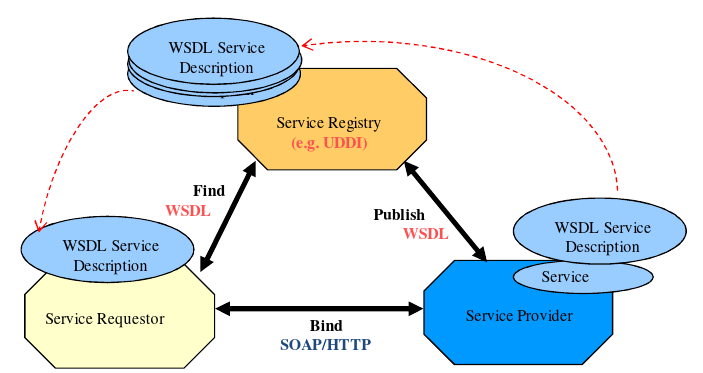
\includegraphics[width=0.8\columnwidth]{fundamentacao/webservice_soap_model} 
  \caption{Modelo de serviço Web baseado em SOAP.\cite{Belqasmi:2011}} 
  \label{fig:wsmodelsoap}
\end{figure}

\begin{itemize}
\item Provedor (Service Provider) - cria e oferece o serviço Web, este precisa descrever o serviço em um formato padrão, neste caso WSDL e, publica-o (\textit{Publish}) no Registro de serviço.
\item Registro de serviço (Service Registry) - contém a descrição publicada pelo Provedor. O registro de serviço mais utilizado é o \textit{Universal Description, Discovery and Integration} (UDDI), este em suas especificações define um conjunto de \textit{Application Program Interfaces}(APIs) tanto para publicação, quanto para descoberta\cite{Belqasmi:2011}.
\item Consumidor (Service Requestor) - obtém informações do registro, \textit{Find}, e utiliza a descrição do serviço capturada para invocar (\textit{Bind}) o serviço Web.
\end{itemize}

A descrição realizada da Figura \ref{fig:wsmodelsoap} foi na verdade a descrição das 3 regras fundamentais do Service Oriented Architecture (SOA), que é um caminho lógico para projetar sistemas de software, os quais podem prover serviços tanto para o usuário final de aplicações quanto para outros serviços distribuídos na rede, através de interfaces que possam ser publicadas e descobertas.\cite{Papazoglou:2008}

Existe também outro tipo de abordagem de serviços Web, baseada nos princípios arquiteturais REST (ver seção \ref{subsec:restful}).

\subsection{SOAP}
\label{subsec:soap}
SOAP é um protocolo leve que foi desenvolvido com a intenção de prover troca de mensagens estruturadas em um ambiente descentralizado e distribuído. Este usa a tecnologia XML para definir um framework extensível de mensagens, o qual permite a construção de mensagens que podem ser trocadas através de uma variedade de protocolos subjacentes. O framework foi desenvolvido para ser independente de modelo de linguagem de programação ou qualquer outra implementação semântica\cite{w3c:soap}. Diz-se que é um protocolo leve pelo fato de somente receber e enviar pacotes de protocolos de transportes (por exemplo, HTTP) e, processar as mensagens XML, quando contrastados com os protocolos ORPC**\cite{Papazoglou_slides:2008}. A figura \ref{fig:wsmodelsoap_expanded} seguinte mostra como o SOAP atua no modelo de serviço Web baseado em SOAP (ver Figura \ref{fig:wsmodelsoap}). Nesta, o \textit{SOAP-based middleware} converte as chamadas de procedimento de/para mensagens XML que são enviadas através do HTTP ou outro protocolo.

\begin{figure}[!htb] \centering 
  \centering
  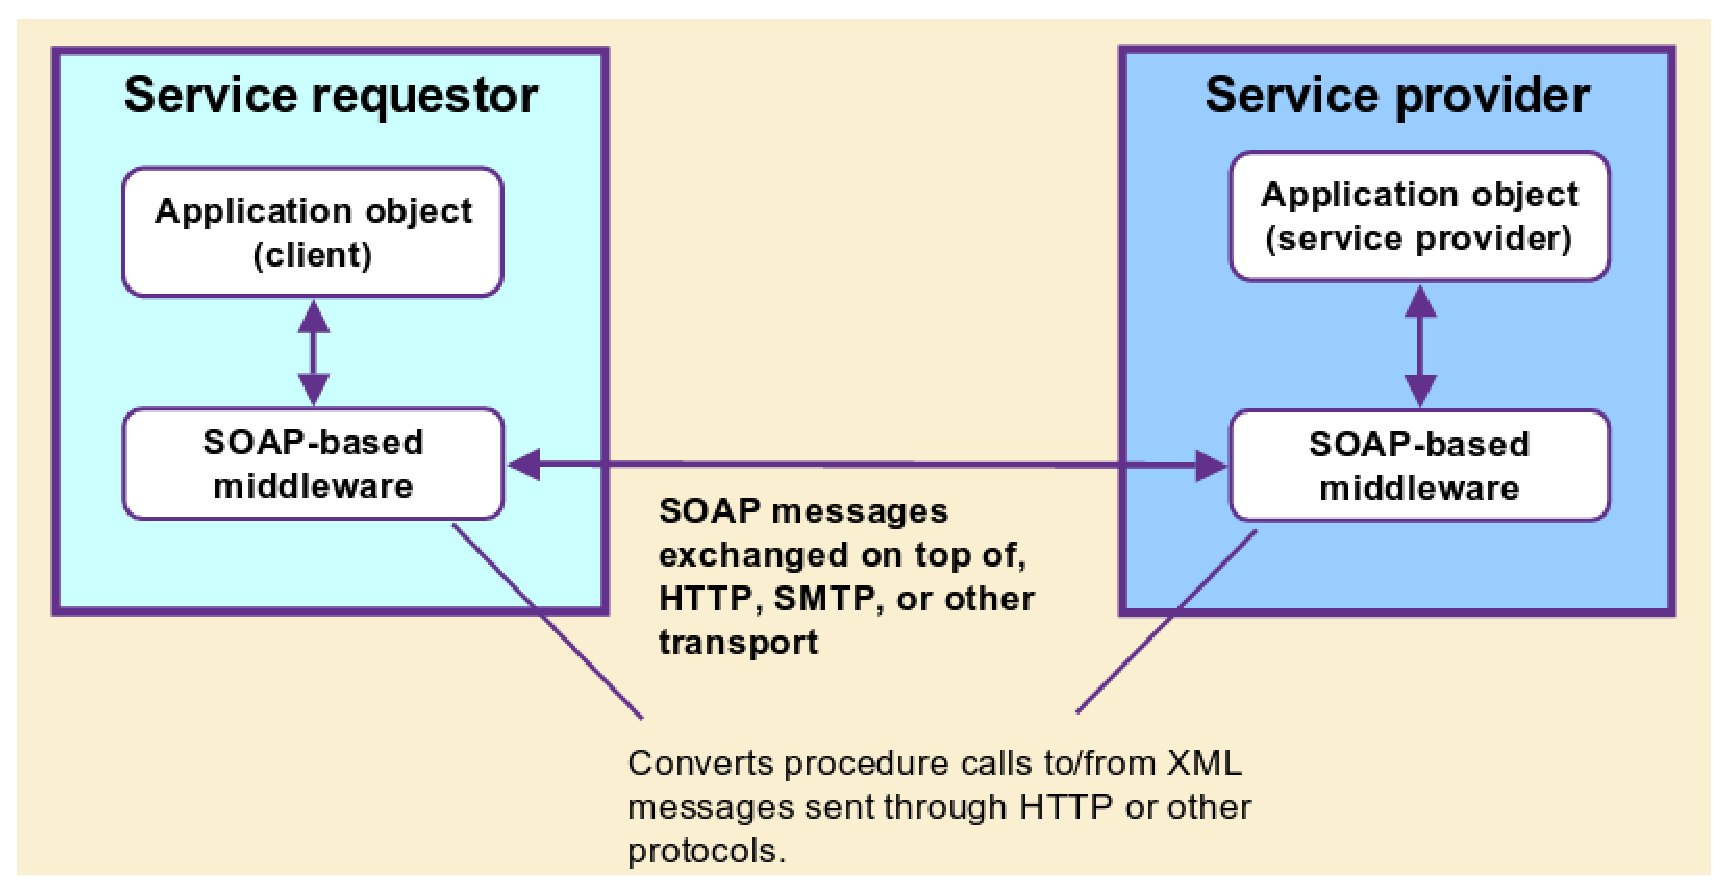
\includegraphics[width=0.8\columnwidth]{fundamentacao/webservice_soap_model_expanded} 
  \caption{SOAP no modelo Modelo de serviço Web baseado em SOAP.\cite{Papazoglou_slides:2008}} 
  \label{fig:wsmodelsoap_expanded}
\end{figure}

Em outras palavras, SOAP é um protocolo de rede de aplicação utilizado para transferir mensagens entre instâncias de serviços descritas por interfaces WSDL (ver Figura \ref{fig:wsmodelsoap_communication_msg}).

Um documento XML SOAP é chamado de SOAP mensagem (ou SOAP envelope) e é usualmente transportado sobre outros protocolos de aplicação, mais frequentemente o HTTP. Mas existem outros protocolos de aplicação que podem ser utilizados: SMTP**, FTP**, RMI**. A mensagem SOAP, representada na Figura \ref{fig:wsmodelsoap_communication_msg} é colocada no corpo da mensagem HTTP e então é encaminhada para seu destino. Na próxima camada, da hierarquia ilustrada na figura e no modelo OSI** (camada de transporte), a mensagem HTTP torna-se segmentos de bytes a serem enviados através do stream do TCP. Do outro lado (destinatário) um \textit{HTTP listener}(fica a espera de novas mensagens) passa o corpo da mensagem HTTP para um processador de mensagens SOAP, o qual entende a sintaxe das mensagens e então é capaz de processá-las.\cite{Papazoglou:2008}
 
\begin{figure}[!htb] \centering 
  \centering
  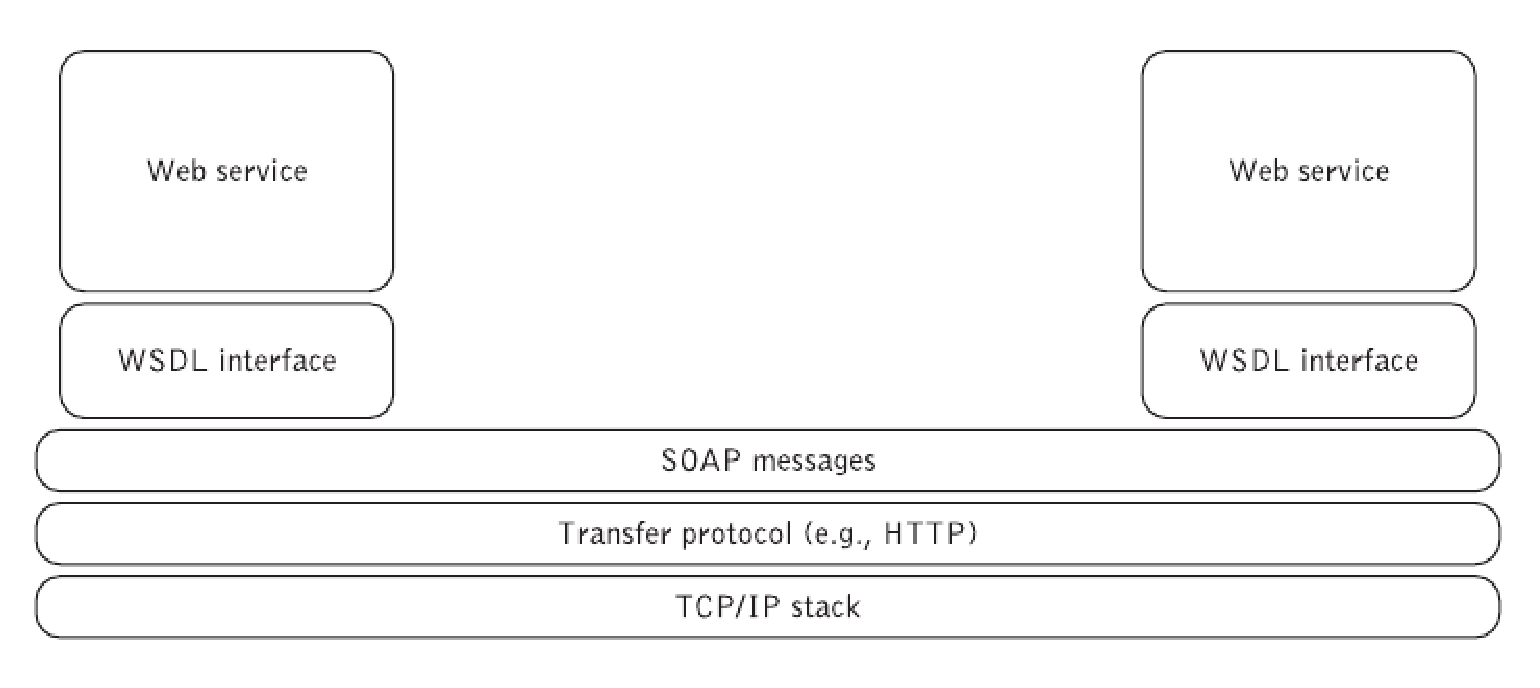
\includegraphics[width=0.8\columnwidth]{fundamentacao/webservice_soap_message_communication} 
  \caption{Comunicação dos serviços Web e mensagem SOAP.\cite{Papazoglou:2008}} 
  \label{fig:wsmodelsoap_communication_msg}
\end{figure}

Uma mensagem SOAP (ver Figura \ref{fig:wssoap_msg}) é composta de um elemento \textless Envelope\textgreater (elemento raiz), o qual contém um \textless Header\textgreater (opcional) e um obrigatório \textless Body\textgreater. Caso um \textless Header\textgreater seja utilizado, este deve ser um filho imediato de \textless Envelope\textgreater, e preceder o \textless Body\textgreater. \textless Body\textgreater contém os dados principais da aplicação (dados arbitrários em um XML ou parâmetros para uma chamada de método). Uma mensagem SOAP pode ter uma declaração XML, \textless ?xml version=``1.0'' encoding=``UTF-8''?\textgreater, a qual indica a versão do XML usado e o formato da codificação. Para que a tag \textless env:Header ou Body ou Envelope\textgreater seja identificada como pertencente ao SOAP \textit{namespace}, esta deve ser referenciada ao SOAP \textit{namespace} URI, xmlns:env=``http://www.w3.org/2003/05/soap-envelope''. Se uma aplicação SOAP recebe uma mensagem que é baseada em outro \textit{namespace}, isto gerará um erro.\cite{Papazoglou:2008}

\begin{figure}[!htb] \centering
  \centering
  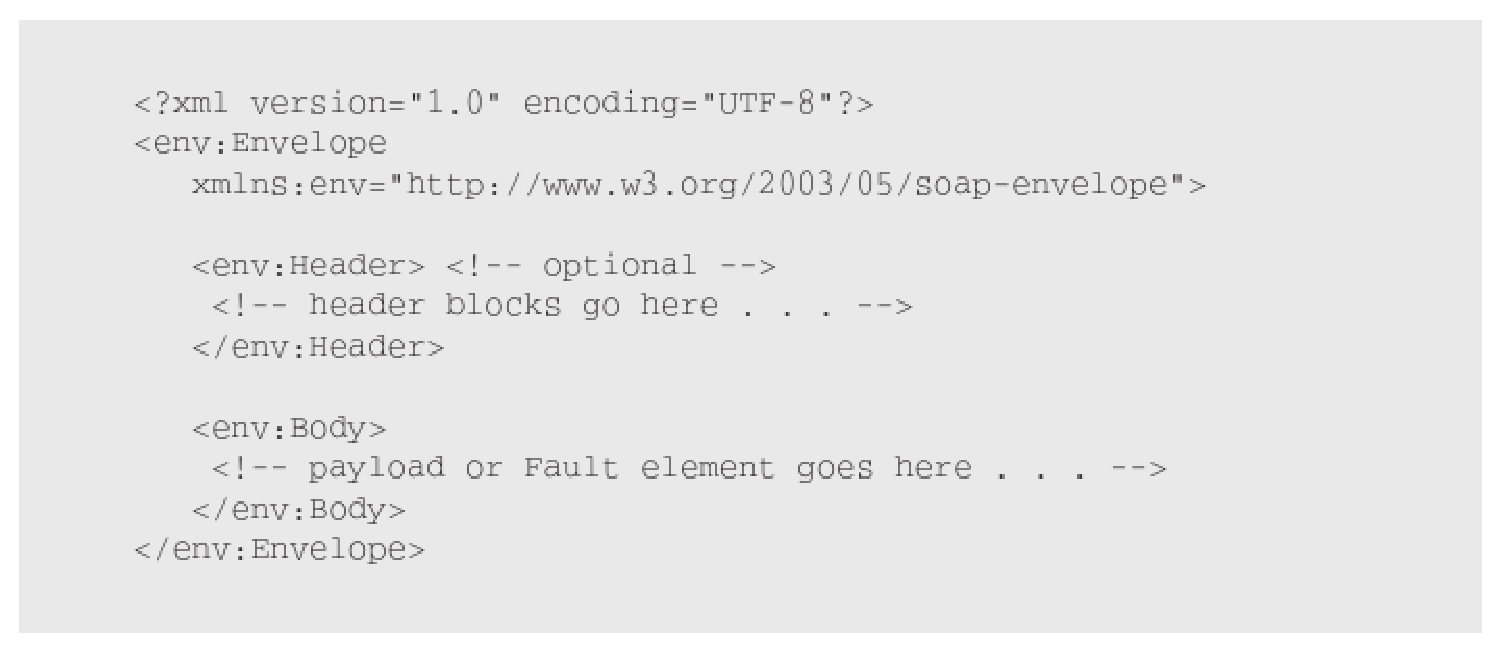
\includegraphics[width=0.8\columnwidth]{fundamentacao/webservice_soap_message_structure} 
  \caption{Estrutura da mensagem SOAP.\cite{Papazoglou:2008}} 
  \label{fig:wssoap_msg}
\end{figure}

O envelope SOAP pode especificar um conjunto de regras que serializam os dados XML da aplicação. Assim, tanto o Provedor quanto o Consumidor devem concordar com as regras de codificação (normalmente baixando o mesmo esquema XML que define eles). Para tal finalidade ambos podem utilizar-se do atributo global(pode ser declarado em qualquer nível do documento XML) \textit{encodingStyle}, este define qual estilo de codificação deve ser utilizado no elemento no qual foi definido e em seus filhos (ver Figura \ref{fig:wssoap_msg_ecodingStyle}). Com o intuito de favorecer a flexibilidade SOAP permite que as aplicações definam seu próprio estilo de codificação, mas na maioria dos casos as regras de codificação padrão são indicadas.\cite{Papazoglou:2008}

\begin{figure}[!htb] \centering
  \centering
  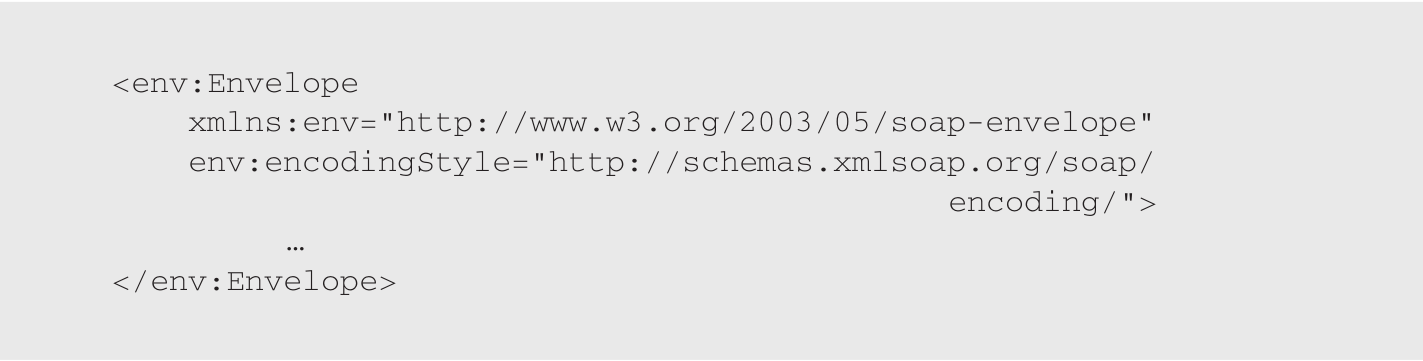
\includegraphics[width=0.8\columnwidth]{fundamentacao/webservice_soap_message_structure_ecodingStyle} 
  \caption{Estrutura da mensagem SOAP com declaração do atributo encodingStyle.\cite{Papazoglou:2008}} 
  \label{fig:wssoap_msg_ecodingStyle}
\end{figure}

O envelope SOAP pode conter no máximo um elemento \textless Header\textgreater, o qual contém todas as dicas que são relevantes para seus destinatários finais ou pontos de transporte intermediários. Também pode conter informação de onde o documento deve ser encaminhado, origem, e pode conter assinaturas digitais. O propósito do \textless Header\textgreater é encapsular extensões ao formato da mensagem sem combiná-las aos dados principais de carga da aplicação ou modificar a estrutura fundamental SOAP. Isto permite adição de especificações de características e funcionalidades, tais como segurança, transporte, referências a objetos, atributos QoS**, dentre outros, sem quebra das especificações da mensagem SOAP. Cada bloco dentro do \textless Header\textgreater deve ter seu próprio \textit{namespace}, assim como já explanado anteriormente, o \textit{namespace} permite que as aplicações SOAP identifiquem o bloco e os processe de acordo com as regras definidas no \textit{namespace} em questão(ver Figura \ref{fig:wssoap_msg_header}).\cite{Papazoglou:2008}

\begin{figure}[!htb] \centering
  \centering
  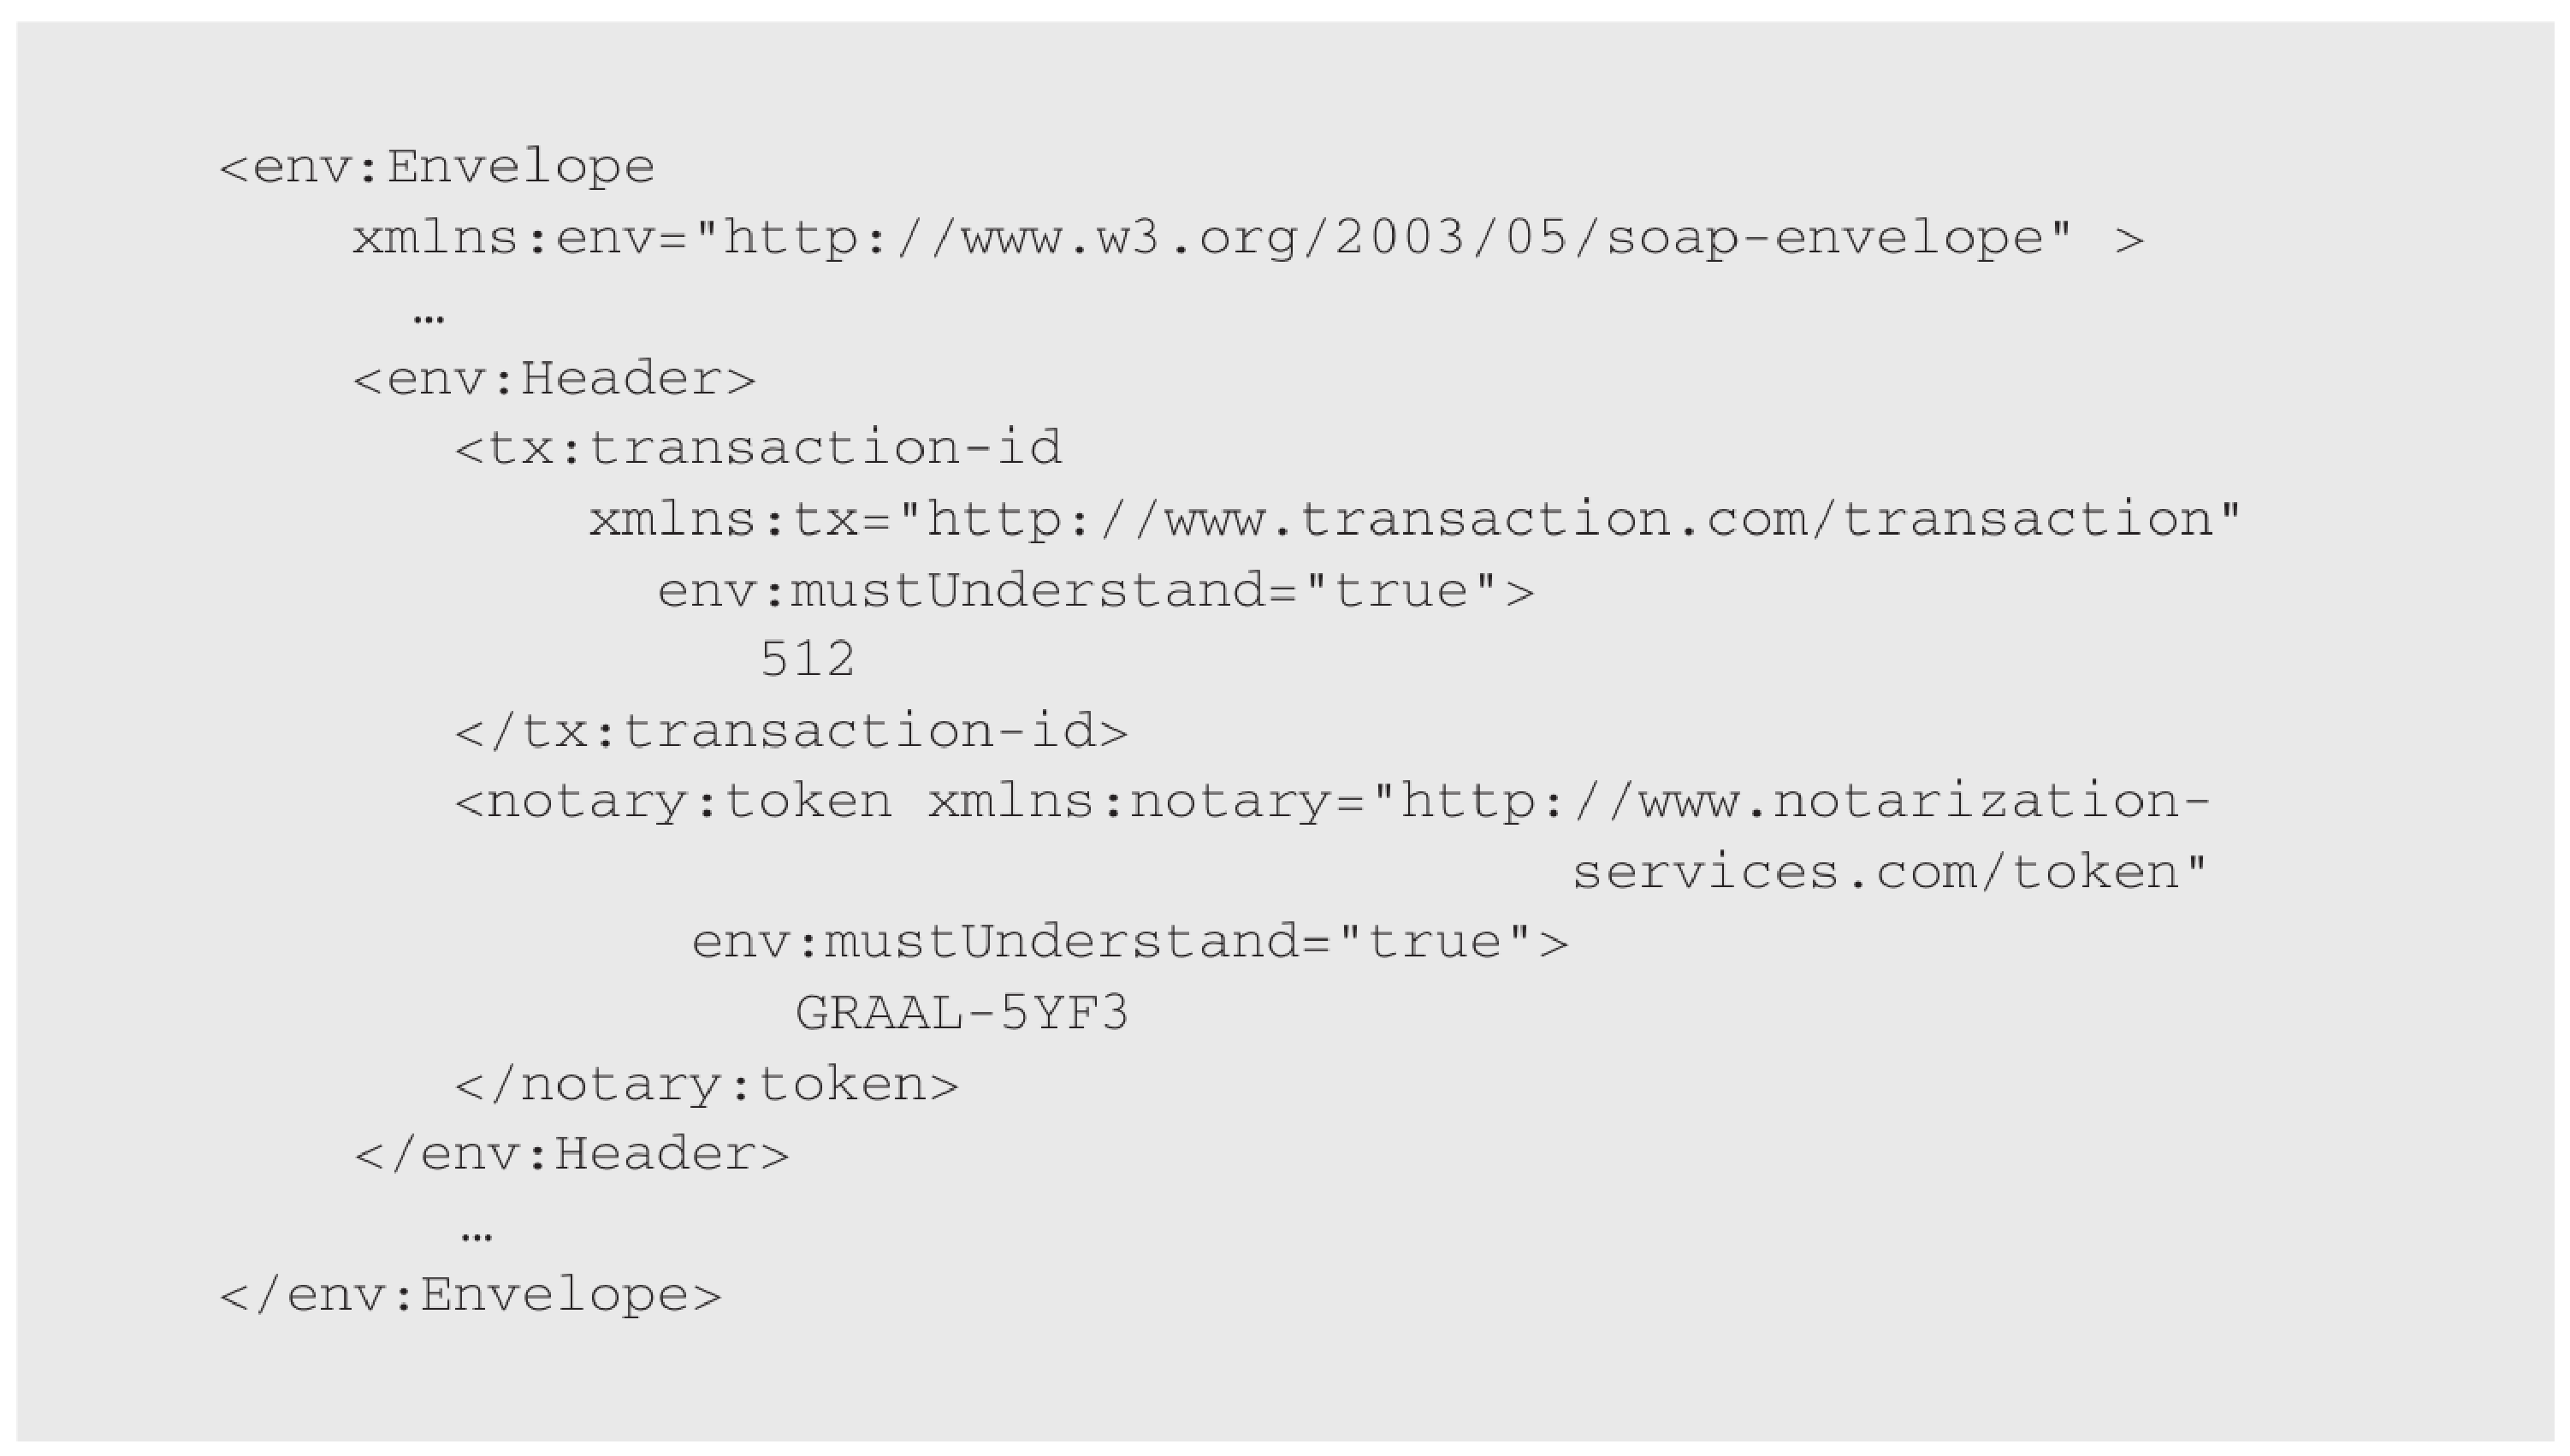
\includegraphics[width=0.8\columnwidth]{fundamentacao/webservice_soap_message_structure_header} 
  \caption{Estrutura da mensagem SOAP, Header.\cite{Papazoglou:2008}} 
  \label{fig:wssoap_msg_header}
\end{figure}

O \textless Body\textgreater pode ter um número arbitrário de filhos (chamados de entradas do \textless Body\textgreater), como também pode conter nenhum. Todas as entradas do \textless Body\textgreater que são filhos imediatos devem ter o \textit{namespace}. Por padrão, o conteúdo do \textless Body\textgreater pode ser um XML qualquer sem especificação de regras. \textless Body\textgreater ou contém os dados principais da aplicação ou uma mensagem de erro, mas não os dois. Ou ainda pode ser vazio.\cite{Papazoglou:2008}

SOAP suporta dois tipos de estilo de comunicação, RPC (Remote Procedure Call) e documento (ou mensagem). Numa comunicação no estilo RPC/Literal, o cliente expressa sua requisição como uma chamada de método passando um conjunto de parâmetros. O método então retorna uma resposta. Algumas regras devem ser seguidas e são exemplificadas na Figura \ref{fig:wssoap_msg_soap_rpc}:
\begin{itemize}
\item \begin{verbatim}Uma URI deve identificar o endereço de destino onde o método será chamado, que pode ser identificado na declaração da tag \textless Envelope\textgreater, xmlns:m=``http://www.plastics_supply.com/product-prices''.\end{verbatim}
\item \begin{verbatim}Deve ser passado o nome do método, \textless m:GetProductPriceResponse\textgreater e, seus parâmetros (nome e valor) na ordem correta que aparece no método a ser chamado, como exemplificado na figura em \textless product-id\textgreater 450R6OP \textless product-id \textgreater.\end{verbatim}
\item \begin{verbatim}Uma mensagem de resposta RPC deve conter um valor de retorno e quaisquer parâmetros de saída ou um erro. Esta é modelada como uma estrutura única com um campo para cada parâmetro na assinatura do método, exemplificado em \textless product-price\textgreater 134.32 \textless product-price\textgreater.\end{verbatim} 
\end{itemize}

\begin{figure}[!htb] \centering
  \centering
  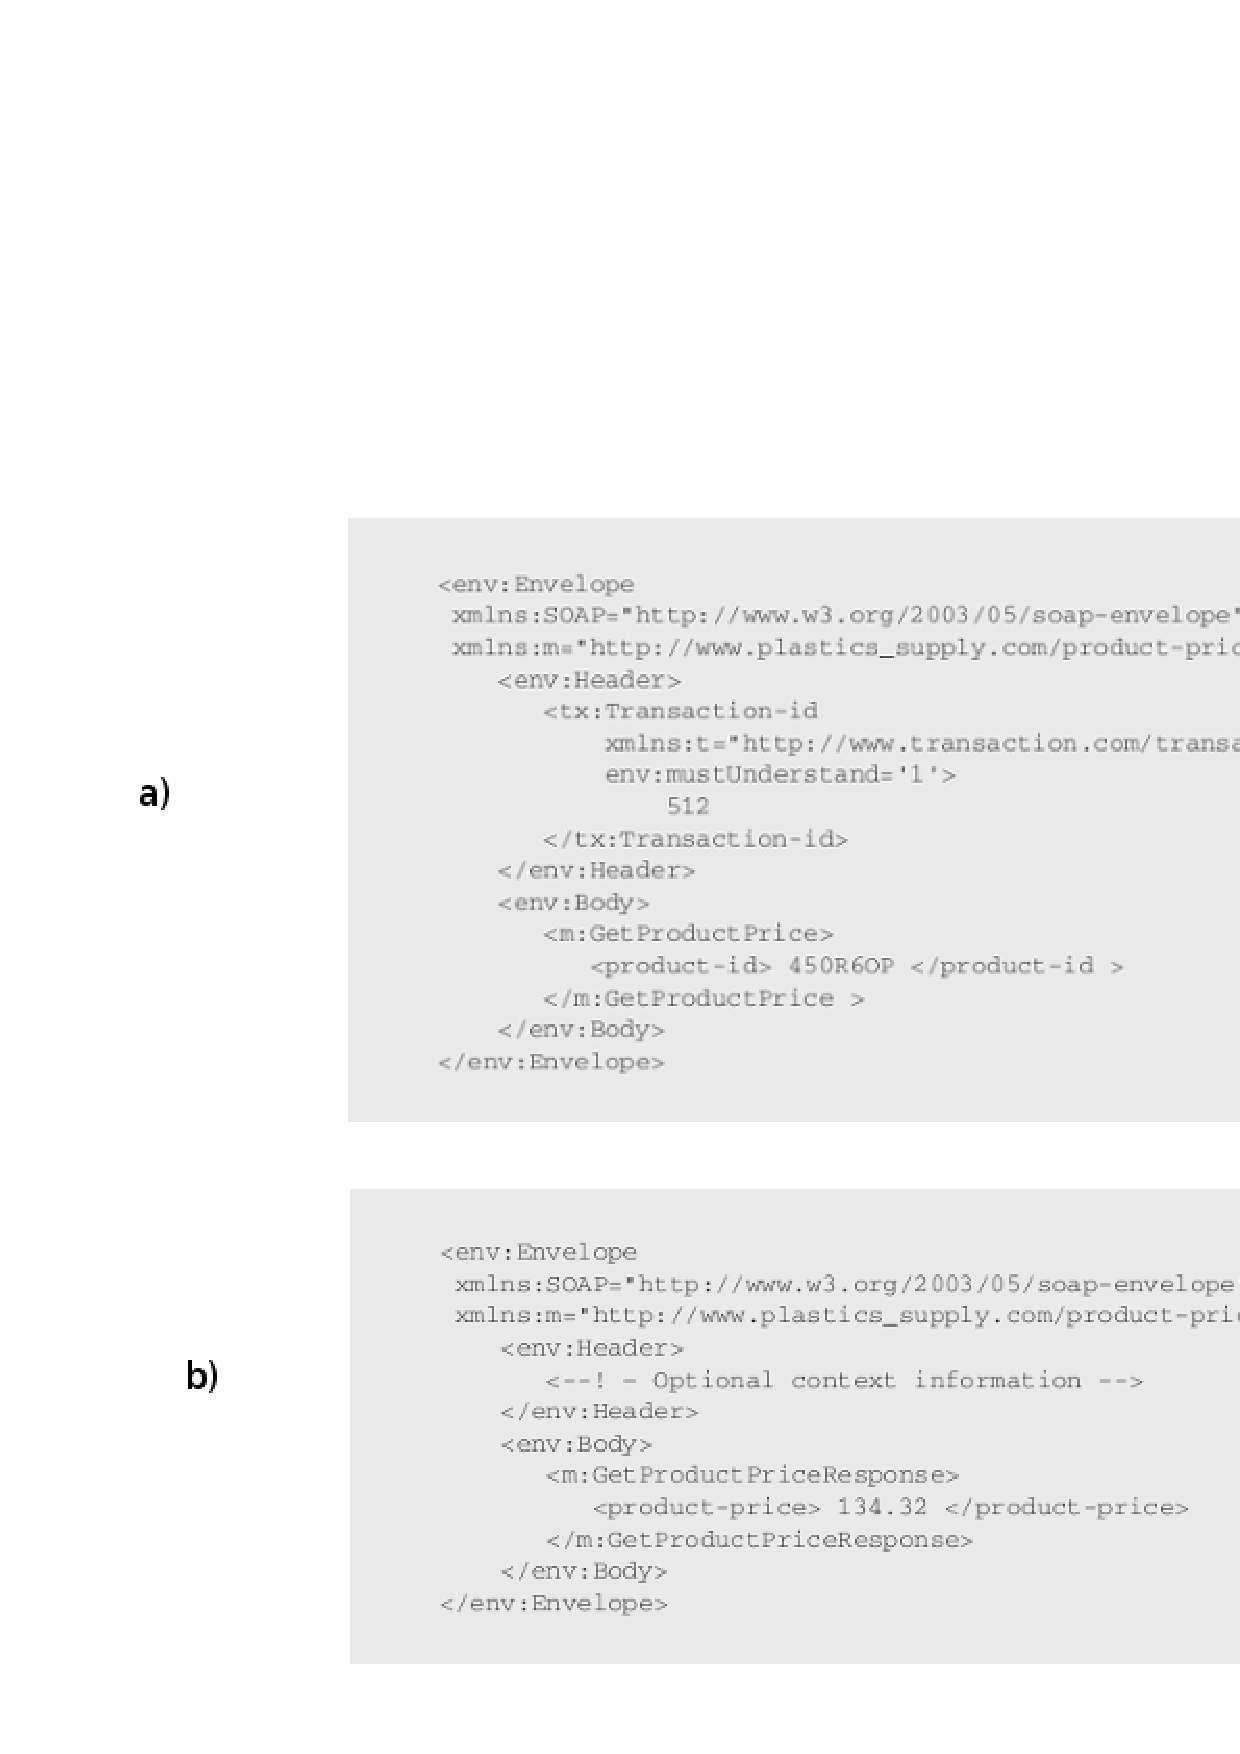
\includegraphics[width=0.8\columnwidth]{fundamentacao/soap_rpc_style} 
  \caption{a)Estilo SOAP RPC \textless Body\textgreater. b) Estilo SOAP RPC \textless Body\textgreater - resposta\cite{Papazoglou:2008}} 
  \label{fig:wssoap_msg_soap_rpc}
\end{figure}

Em uma comunicação no estilo documento, SOAP é utilizado para trocar documentos contendo qualquer tipo de dados XML no \textless Body\textgreater, com o XML não codificado. No estilo de mensagem \textit{Document/Literal}, o \textless Body\textgreater contém um elemento XML bem formado com dados da aplicação de qualquer tipo. O ambiente de execução SOAP aceita o elemento \textless Body\textgreater da maneira com que chegou e o trata sobre a aplicação a qual foi destinado. Pode ou não ter uma resposta associado com a mensagem. A Figura \ref{fig:wssoap_msg_soap_document} é um exemplo de mensagem neste estilo, a qual exemplifica os dados de um pedido de compra. Observa-se que este tipo de envio de dados não é muito bem conduzido para o estilo RPC, como o demonstrado na Figura \ref{fig:wssoap_msg_soap_rpc}. Em vez disso, a aplicação almeja transferir os dados da aplicação de uma única vez a um serviço para processamento futuro.\cite{Papazoglou:2008}

\begin{figure}[!htb] \centering
  \centering
  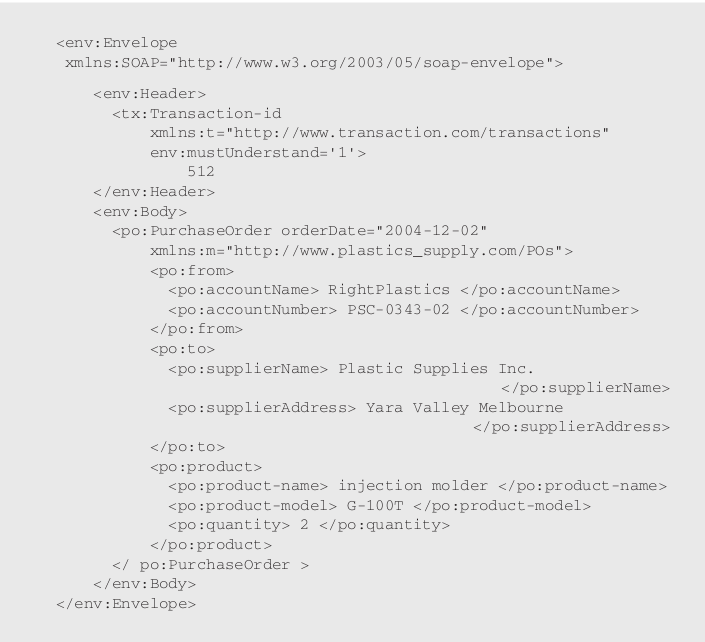
\includegraphics[width=0.8\columnwidth]{fundamentacao/soap_document_style} 
  \caption{Exemplo de um \textless Body\textgreater no estilo documento SOAP.\cite{Papazoglou:2008}} 
  \label{fig:wssoap_msg_soap_document}
\end{figure}

As requisições SOAP normalmente utilizam o protocolo de transporte HTTP. Quando utilizado as requisições SOAP são transportadas dentro do corpo do método POST do HTTP e suas respostas são retornadas nas respostas do HTTP (ver Figuras \ref{fig:wssoap_soap_http_request_rpc} e \ref{fig:wssoap_soap_http_response_rpc}).

\begin{figure}[!htb] \centering
  \centering
  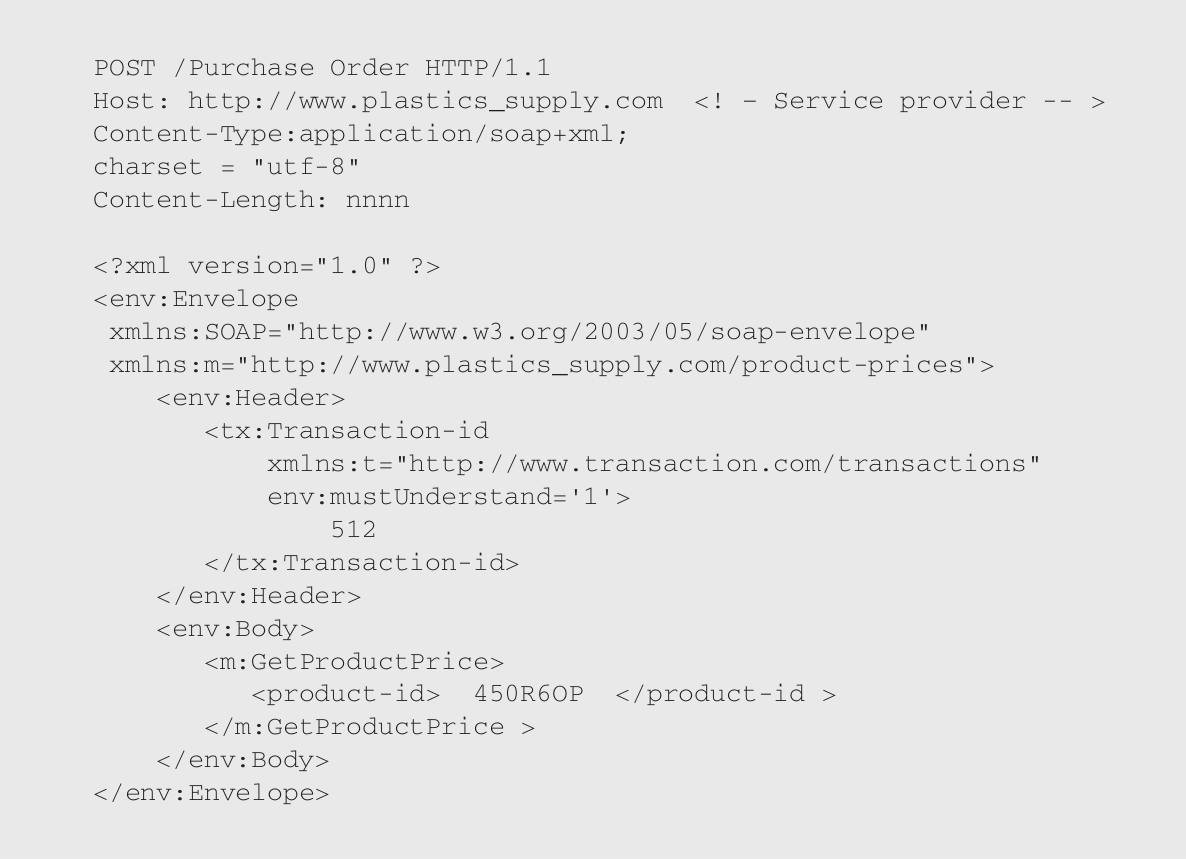
\includegraphics[width=0.8\columnwidth]{fundamentacao/soap_http_request_rpc} 
  \caption{Requisição SOAP no estilo RPC dentro do corpo da requisição HTTP.\cite{Papazoglou:2008}} 
  \label{fig:wssoap_soap_http_request_rpc}
\end{figure}

\begin{figure}[!htb] \centering
  \centering
  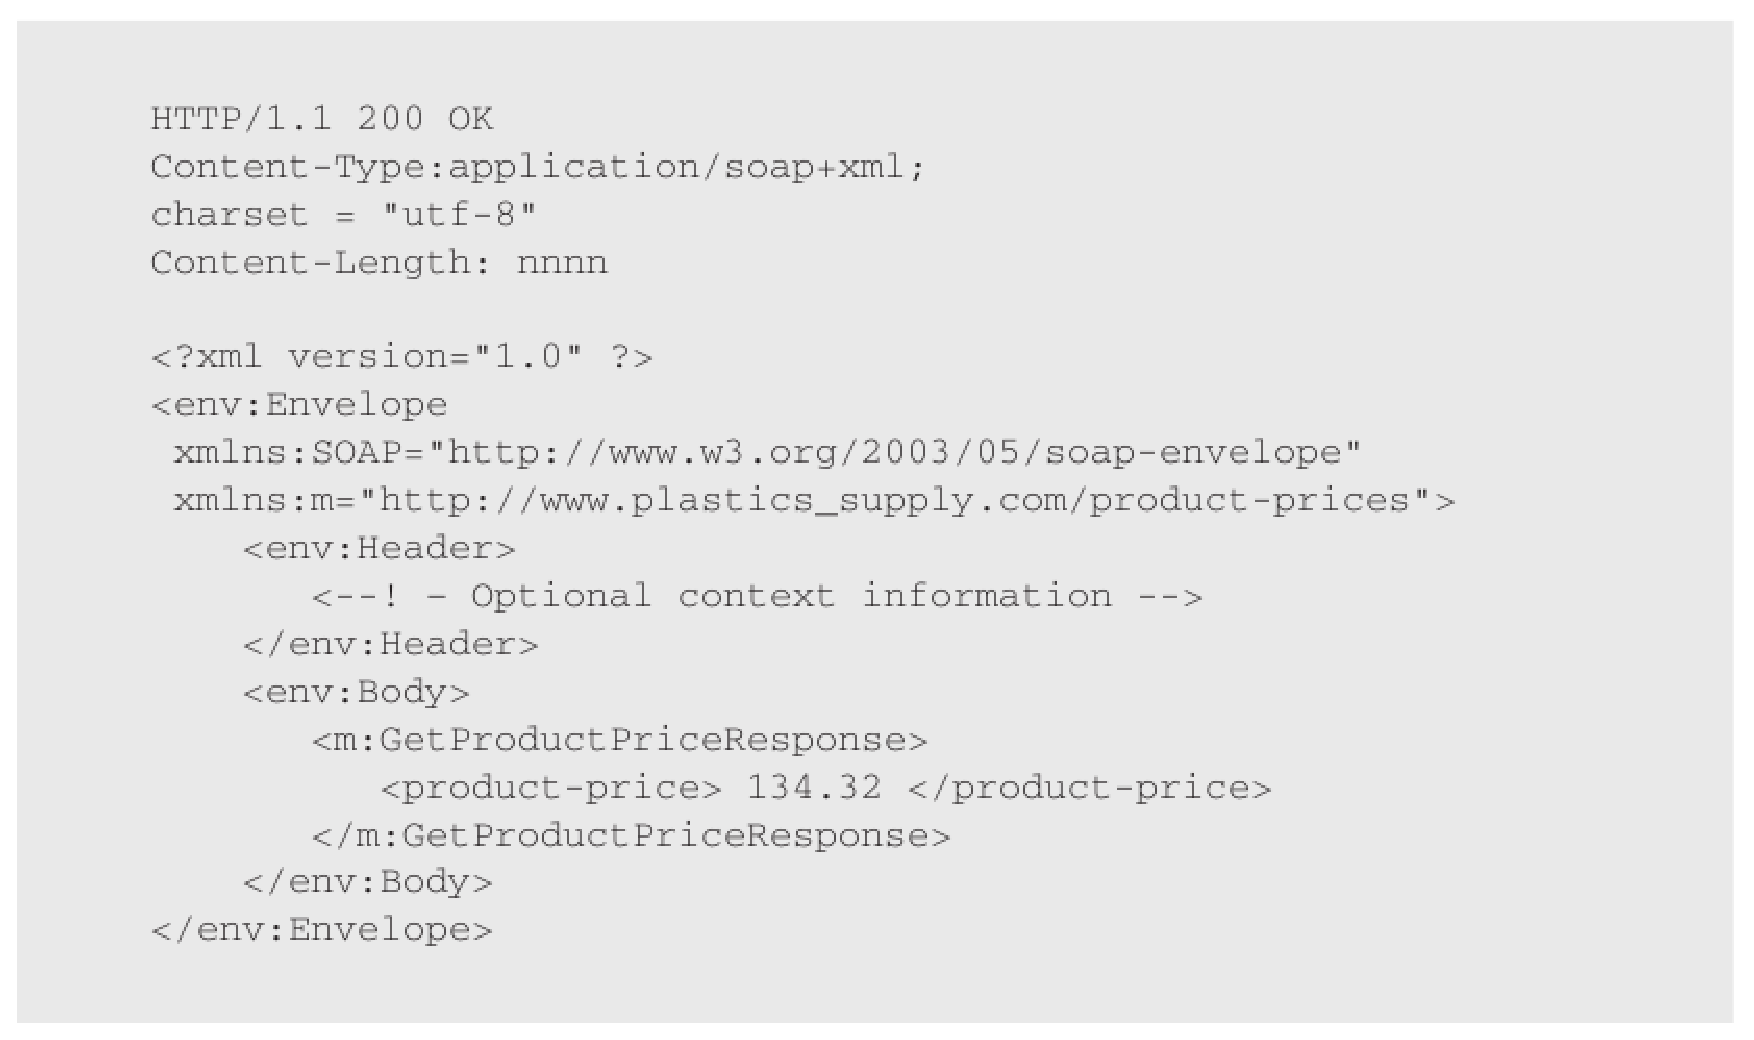
\includegraphics[width=0.8\columnwidth]{fundamentacao/soap_http_response_rpc} 
  \caption{Resposta SOAP no estilo RPC dentro do corpo da resposta HTTP.\cite{Papazoglou:2008}} 
  \label{fig:wssoap_soap_http_response_rpc}
\end{figure}

\subsection{Serviços Web RESTFul}
\label{subsec:restful}
Segundo \cite{Heffelfinger:2014}, Representational State Transfer (REST) é um estilo de arquitetura no qual serviços Web são vistos como recursos e podem ser identificados por Uniform Resources Identifiers (URIs). Serviços Web que são desenvolvidos usando REST são conhecidos como RESTful web services. 

Os principais princípios do estilo arquitetural REST são: endereçamento global através de identificação dos recursos, interface uniforme compartilhada por todos os recursos, interações \textit{stateless} entre os serviços, mensagens auto-descritivas e \textit{hypermedia} como um mecanismo para descoberta descentralizada de recursos por referência\cite{Pautasso:2014}. Na lista abaixo se têm uma explanação a respeito dos princípios citados.

\begin{enumerate}
\item Identificação dos recursos - todos os recursos que são publicados por um serviço Web deveriam ser disponibilizados por um único e estável identificador global\cite{Pautasso:2014}. A exemplo das URIs\cite{Franca:2011}.
\item Interface uniforme - todos os recursos interagem através de uma interface uniforme, a qual prover um conjunto de métodos pequeno, genérico e funcionalmente suficiente para suportar todas as possíveis interações entre os serviços. Cada método tem uma semântica bem definida em relação aos efeitos que causará no estado do recurso. No contexto da Web e do protocolo HTTP que é utilizado, ``Interface uniforme'' pode ser alcançado com os seus  métodos(GET, PUT, DELETE, POST, HEAD, OPTIONS, dentre outros) os quais podem ser aplicados para todos os identificadores dos recursos Web (URIs).\cite{Pautasso:2014}
\item Interações \textit{stateless} - os serviços não podem estabelecer sessões permanentes entre eles. Isto assegura que as requisições para um recurso sejam independentes entre si. No final de cada interação, não há estados compartilhados entre clientes e servidores. Requisições podem resultar em uma mudança de estado do recurso, mas o novo estado é imediatamente visível para todos clientes.\cite{Pautasso:2014}
\item Mensagens auto-descritivas - Serviços interagem através de requisição e mensagem de resposta, que contem tanto os dados (representações dos recursos) e correspondente \textit{meta-data}. As representações podem variar de acordo com o contexto do cliente, interesses e habilidades. Por exemplo, um cliente \textit{mobile} pode obter uma representação do recurso que exige pouco consumo de banda de dados. Da mesma forma, um navegador pode requisitar a representação de uma página Web em uma linguagem específica, de acordo com suas preferências. Esta característica aumenta de maneira significativa o grau de interoperabilidade, pois um cliente pode dinamicamente negociar o mais apropriado formato de representação com o recurso (também conhecido como media type), em vez de ser forçado a sempre trabalhar com uma determinada representação do recurso. As requisições e mensagens de respostas também devem conter explicitamente \textit{meta-data} sobre sua representação, desta maneira os serviços não precisam assumir algum tipo de acordo de sobrecarga no sentido de como tal representação seria analisada, processada e entendida.\cite{Pautasso:2014}
\item \begin{verbatim}\textit{Hypermedia} - Recursos podem ser relacionados entre si. \textit{Hypermedia} embute referências a outros recursos relacionados ou dentro de suas representações ou em sua correspondente \textit{metadata}. Clientes então podem descobrir os \textit{hyper-links} dos recursos relacionados ao processar suas representações e escolher seguir o link. Como exemplificado em \cite{Franca:2011}, um sistema de uma instituição que possui um recurso ``lista_cursos'' (lista todos os cursos da instituição), este pode oferecer os \textit{hyper-links} que representam cada recurso que representa um determinado curso. \textit{Hypermedia} auxilia na descoberta descentralizada de recursos e também pode ser utilizada para descoberta e descrição de protocolos de interação entre os serviços. Pelo fato deste ser o princípio menos utilizado pelas APIs que se dizem ser RESTFul, algumas vezes as APIs disponibilizadas por serviços Web que além das outras restrições contemplam esta, são também chamadas de \textit{Hypermedia APIs}.\cite{Pautasso:2014}\end{verbatim}
\end{enumerate}

\subsection{Dispositivos como serviços Web RESTFul} 
\label{subsec:dispositivosWeb}
Como abordado em \ref{sec:iot} um dos desafios referentes a visão da IoT é sua interoperabilidade e, como possível solução se pode disponibilizar os dispositivos como serviços Web RESTFul. Desta maneira os dispositivos podem interagir entre si e com outros sistemas na Web.

A disponibilização dos dispositivos como serviços Web RESTFul vêm sendo empregada através de duas abordagens. Na primeira, quando os dispositivos têm recursos suficientes (memória, processamento e largura de banda de rede) servidores Web são embarcados nos próprios dispositivos e estes são disponibilizados como recursos REST. Enquanto que na segunda, quando uma coisa não possui recursos suficientes para tal propósito, utiliza-se de outro dispositivo, por exemplo, um \footnotemark{Raspberry Pi}\footnotetext{**} ou qualquer outro controlador com recursos suficientes para instalação e execução de um servidor Web. Este então atua como um intermediador entre o objeto e a Internet oferecendo a coisa como um recurso REST.\cite{Franca:2011}

Adotando esse padrão, os dispositivos podem ter suas propriedades disponíveis através de qualquer navegador, sem a necessidade de instalação de nenhum programa ou driver adicional, como pode ser exemplificado na Figura \ref{fig:dispnavegador}. Além disto, mashups físicos\footnotemark \footnotetext{Aplicativos criados a partir da composição de dados e serviços de dispositivos físicos com outros recursos Web.} podem ser construídos com muito menos esforço do que as existentes abordagens, quebrando drasticamente a barreira para o desenvolvimento de aplicações com dispositivos\cite{Guinard:2009}. Pelo fato das coisas serem disponibilizadas como serviços Web, ainda pode-se utilizar-se dos outros recursos disponíveis na Web, a exemplo de sistemas de cache, balanceamento de carga, indexação e, pesquisa\cite{Franca:2011}. Assim então promovendo a visão da Internet das Coisas.

\begin{figure}[!htb] \centering 
  \centering
  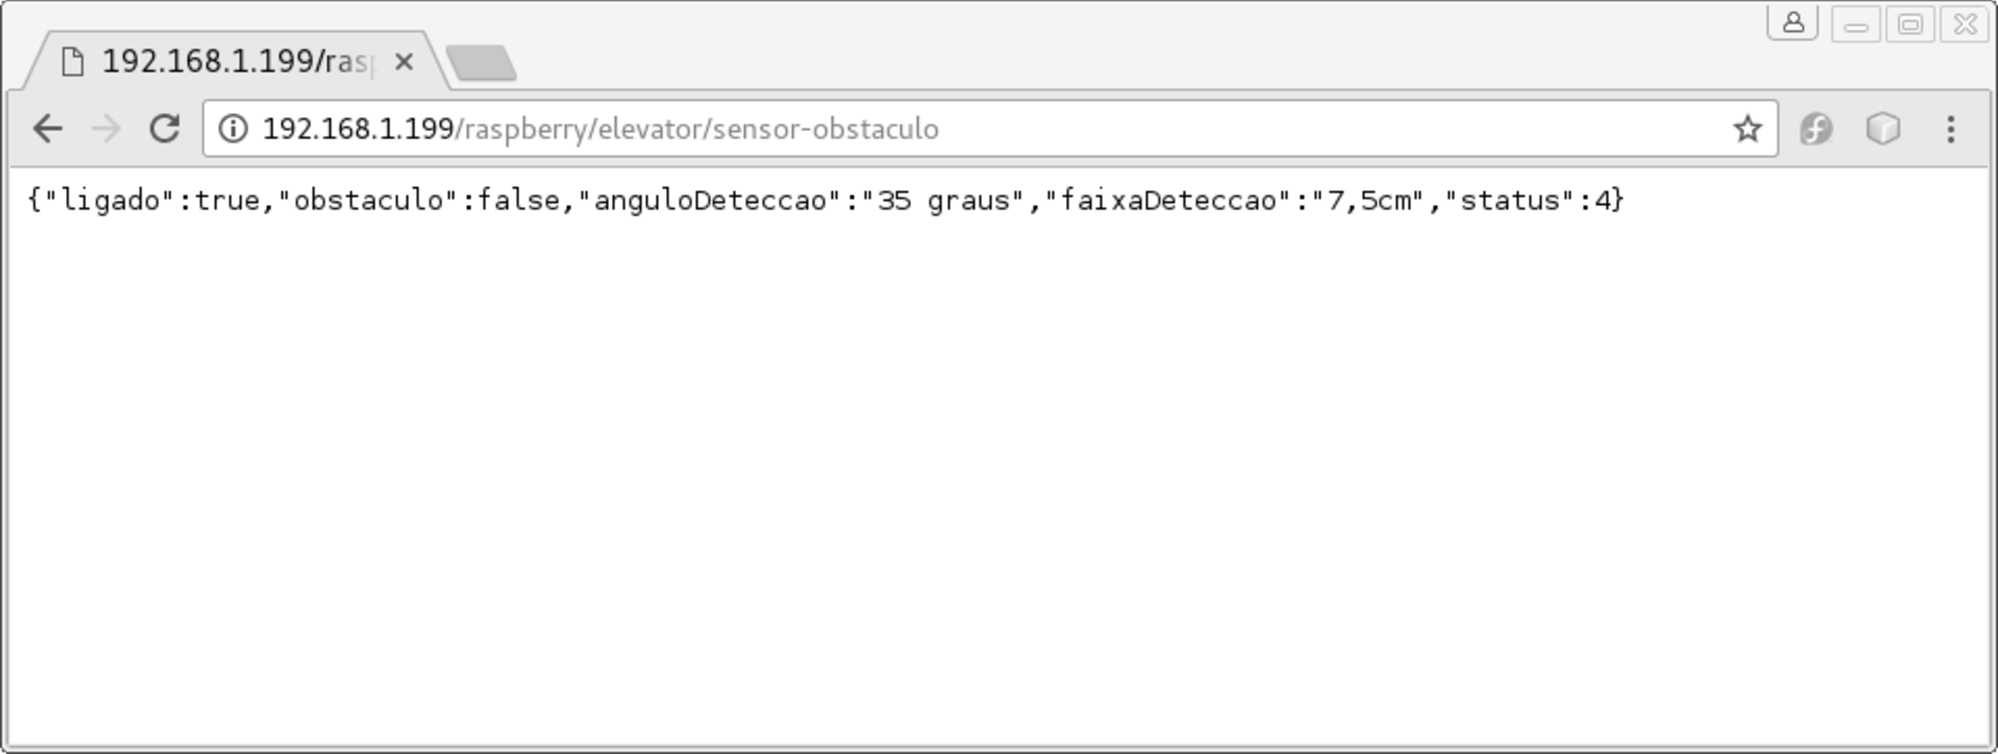
\includegraphics[width=0.8\columnwidth]{fundamentacao/elevator_sensor_example} 
  \caption{Dispositivo sensor de obstáculo do elevador disponibilizado como serviço. Faixa de detecção compatível com a largura do elevador utilizado na maquete do experimento    \ref{ch:experimento}} 
  \label{fig:dispnavegador}
\end{figure}

No cenário da IoT os princípios REST têm sido amplamente aplicados na integração dos dispositivos inteligentes a Web, pois esses princípios parecem ser mais adequados para dispositivos com poucos recursos de hardware\cite{Franca:2011}. Para deixar claro os motivos da adoção do REST para disponibilização de dispositivos como serviços Web ao invés dos serviços Web baseados em SOAP, será realizada uma comparação a seguir.

Uma das diferenças entre o REST e WS-* SOAP está na forma como o protocolo HTTP é empregado. Com REST, o HTTP é utilizado para prover interfaces uniformes onde cada método (GET, PUT, DELETE, POST, HEAD, OPTIONS, dentre outros) tem uma semântica bem definida em relação aos efeitos que causará no estado do recurso\cite{Franca:2011}, enquanto que nos WS-* SOAP cada serviço tem seu próprio conjunto de operações explicitamente declarados dentro de um documento WSDL\cite{Pautasso:2014}. O SOAP utiliza o HTTP como um protocolo de transporte (HTTP é um protocolo da camada de aplicação de rede). As mensagens SOAP são adicionadas ao corpo do HTTP. Nos WS-* SOAP o método POST do HTTP é utilizado na troca de mensagens entre cliente e servidor e, a informação sobre qual funcionalidade deve ser executada está presente na mensagem SOAP e não na requisição HTTP. Os serviços Web baseados em SOAP utilizam a Web como meio de troca de mensagens, enquanto os serviços Web RESTFul são parte da Web, ou seja, é visto como um terreno comum para as aplicações\cite{Franca:2011}.

O formato da mensagem SOAP ocasiona um maior consumo de banda devido ao tamanho da mensagem SOAP (ver Figura \ref{fig:msg_soapXrest}), um dos principais motivos para utilizar dispositivos como serviços Web RESTFul, pois muitos dispositivos na IoT possuem baixa capacidade de processamento e de banda de rede. Além disso, este formato pré-definido de mensagem força o cliente a tratar sempre este tipo de mensagem, enquanto utilizando REST é possível oferecer diferentes tipos de representações (JSON, XML, dentre outros).\cite{Franca:2011}

\begin{figure}[!htb] \centering 
  \centering
  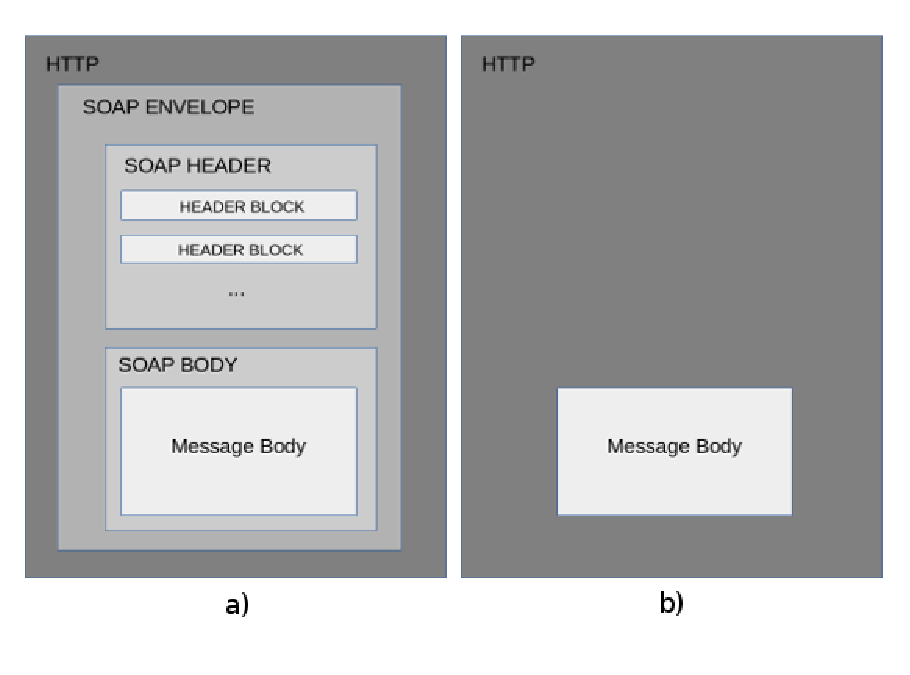
\includegraphics[width=0.8\columnwidth]{fundamentacao/messages_restXsoap} 
  \caption{a)Mensagem SOAP sobre HTTP. b)Mensagem utilizando REST sobre HTTP. Figura baseada em \cite{Pautasso:2014}} 
  \label{fig:msg_soapXrest}
\end{figure}

Tratando o termo ``fraco acoplamento'' somente como a capacidade de fazer modificações no provedor de serviço sem afetar o cliente, os serviços Web RESTFul são menos acoplados, pois as operações sobre os recursos não mudam, já que tais operações são sobre os métodos do HTTP. Uma ressalva é que se as alterações forem feitas nos parâmetros passados nas mensagens, tanto o SOAP quanto o REST estarão no mesmo nível de acoplamento.\cite{Franca:2011}

Por fim, na Figura \ref{fig:comparative_services_soap_rest} é apresentado uma análise comparativa entre duas aplicações que oferecem as mesmas funcionalidades, sendo que uma foi construída utilizando serviços Web SOAP e a outra utilizando serviços Web baseado nos princípios arquiteturais REST. A aplicação em questão é de conferência multimídia e pode ser usada para criar uma conferência, adicionar ou remover um participante de uma conferência que esteja em progresso, atualizar o tipo de mídia (mudar de audio para vídeo) e deletar uma conferência. Ambas as aplicações foram desenvolvidas em um mesmo ambiente e foram publicadas em um mesmo servidor de aplicação. Vários cenários foram executados e performances foram medidas. Todas as medidas são de tempo (milissegundos) e cada resultado é a média de 10 experimentos. Observe que tanto na mesma máquina quanto em um ambiente distribuído a performance do REST é sempre melhor, sendo superior de 3 até 5 vezes em relação ao SOAP quando em ambiente distribuído.\cite{Belqasmi:2012}

\begin{figure}[!htb] \centering 
  \centering
  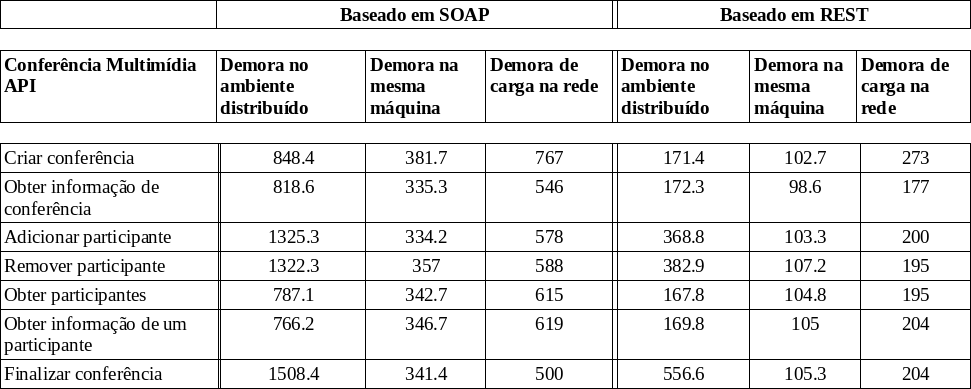
\includegraphics[width=0.8\columnwidth]{fundamentacao/comparative_services_soap_rest} 
  \caption{Resultados de performance entre duas aplicações com mesmas funcionalidades, mas uma baseada em SOAP e outra em REST. Figura adaptada de \cite{Belqasmi:2012}} 
  \label{fig:comparative_services_soap_rest}
\end{figure}

\subsection{Home network system}
\label{sec:hns}
Como explanado anteriormente IoT pode ser descrita como a presença pervasiva de objetos do cotidiano, como \textit{smartphones}, televisores, sensores, dentre outros, que juntos são interligados para prover novas formas de comunicação entre as pessoas e entre os próprios objetos. Observe que tal visão também pode ser empregada dentro do ambiente de uma casa, tornando possível o desenvolvimento de um espaço inteligente, confortável e que promove uma melhor qualidade de vida as pessoas. Diferentes sensores e aparelhos domésticos a exemplo de lâmpadas, ar-condicionadores, sistema de segurança e entretenimento, além de interagirem dentro do ambiente doméstico, podem ser conectados a Internet e controlados por um \textit{smartphone} ou qualquer outro dispositivo da IoT. Desta forma pode-se não só controlar os dispositivos como também monitorar o ambiente doméstico (temperatura, consumo de energia, dentre outros). Uma casa com essas características é comumente chamada de \textit{Smart Home} e é normalmente implementada como um \textit{Home Network System}.\cite{Piyare:2013}

Um \textit{Home Network System} (HNS) é uma rede doméstica de coisas (aparelhos domésticos e sensores) com capacidade de conectividade de rede e, interface de controle e monitoramento. Nesse tipo de sistema os aparelhos e sensores podem juntos prover novas funcionalidades, as quais atendam as expectativas do usuário, como por exemplo, ``Levar compras'' (ver seção \ref{**}). Os aparelhos e sensores dessa rede podem ser disponibilzados como serviços Web RESTFul (ver seção \ref{**}). O HNS tem um componente denominado de \textit{Home Server}, este acessa os dispositivos através de APIs e disponibiliza as funcionalidades ao usuário final. O HS também pode atuar de outra forma, detectando e resolvendo efeitos colaterais indesejáveis (ver sessão\ref{**}), os quais acontecem quando a interação dos dispositivos provoca um estado não esperado no resultado final da operação. O HS com essas características pode ser chamado de \textit{Feature Interaction Manager}. O FIM ou HS, neste caso, ainda pode servir de mediador para redes externas, ou seja, este pode disponibilizar cada serviço de forma única na Internet, para isto, basta o FIM ter um endereço IP público estático e oferecer seus serviços através de uma API, por exemplo, uma API que segue os princípios REST. Desta forma, cada dispositivo do HNS pode ser identificado unicamente na chamada Internet das Coisas. \cite{Nakamura:2009}\cite{Ikegami:2013}

\section{Aprendizado supervisionado}

\subsection{Redes neurais}

\subsection{Métodos avaliativos}
\cite{Witten:2005} pag 183 - livro data mining - parte escrita - 

\section{Interação de características}
TODO....origem...causas...etc...
--Semantic Web-based policy interaction detec method with rules in smart home for detecti interactions among user policies
**interaction among user policies of smart home.

--Feature Interactions in Integrated Services of Networked Home Appliances
--Considering impacts and requirements for better understanding of environment interactions in home network services
**appliance interactions
**environment interactions


Como nesse tipo de sistema, serviços podem ser executados ao mesmo tempo, interação entre Unidades de Funcionalidade de Software (UFS) podem ocorrer e ocasionar efeitos colaterais (ver sessão 6).\cite{Ikegami:2013}
\subsection{Efeitos colaterais desejáveis}
TODO....
\subsection{Efeitos colaterais indesejáveis}
Segundo \cite{Weiss:2007}o problema de efeitos colaterais indesejáveis vem sendo tratado como \textit{the feature interaction problem}.

Em \cite{Weiss}???talvez seja bom mudar esta referencia??? \textit{feature interaction} é definido como a interação entre independentes características***, as quais podem ser intencionais ou não intencionais, podendo levar a efeitos colaterais indesejáveis. Segundo \cite{Weiss:2007 } tais efeitos colaterais indesejáveis podem ser um estado inconsistente do sistema ou inconsistência de dados, tais como, um comportamento não esperado (não desejado), uma quebra de requisito de segurança, dentre outros.


%\xchapter{Trabalhos Relacionados}{Trabalhos relacionados a detecção de efeitos colaterais indesejados na Internet das Coisas}
%\label{ch:related}

%\cite{Wilson:2008} 

Os autores em \cite{Nakamura:2009} apresentam um método de detecção e resolução online para interação de características entre serviços integrados no \textit{Home Network System}. Os atores definem dois tipos de interação de características, \textit{appliance interaction} e \textit{environment interaction}. \textit{Appliance interaction} refere-se a uma situação onde dois serviços compartilham um mesmo dispositivo de forma conflitante, enquanto que \textit{environment interaction} ocorre quando dois serviços, os quais não necessariamente compartilham os mesmos dispositivos, mas conflitam-se por propriedades de ambientes, como por exemplo luminosidade. O método proposto utiliza mecanismos de suspender/resumir, prioridade e tempo de ativação dos serviços para detectar e resolver as interações. Na arquitetura de HNS utilizada, os dispositivos são utilizados para prover serviços ao usuário da casa, e estes são acessados somente pelo HS através das APIs dos dispositivos. Os dispositivos nesta arquitetura não têm capacidade de se comunicar e oferecer serviços entre eles de forma independente. Em outro trabalho mais adiante \cite{Ikegami:2013} deste, no qual Nakamura e Ikegami participaram, estes juntamente com Matsumoto propuseram uma extensão do trabalho anterior. Nesta, os autores definem um modelo (\textit{environment impact model}) o qual define como cada dispositivo contribui para as variáveis de ambiente. Também é introduzido um \textit{environment requirement} para definir o estado esperado de cada serviço. Então  o conceito anterior de environment interaction é reformalizado introduzindo uma condição que uma certa quantidade de impactos acumulados viola os requerimentos dos serviços em questão. O autor realizou cinco casos de estudos os quais conseguiu detectar interações que não tinha conseguido com a definição enterior.

\cite{Maternaghan:2013}
\cite{Alfakeeh:2016}



\xchapter{Abordagem proposta}{//TODO}
\label{ch:proposed}

\section{Cenário}
\label{sec:cenario}
O cenário descrito em \ref{subsec:levarcompras} é idealizado no HNS da Figura \ref{fig:hnsworkmodel}. Neste, cada dispositivo da casa (veículo terrestre, elevador, garra mecânica) é disponibilizado como um serviço Web RESTFul (seção \ref{subsec:dispositivosWeb}). O HS deste cenário é um servidor Web RESTFul com um FIM (seção\ref{sec:featureinteraction}) integrado.

\begin{figure}[!htb] \centering 
  \centering
  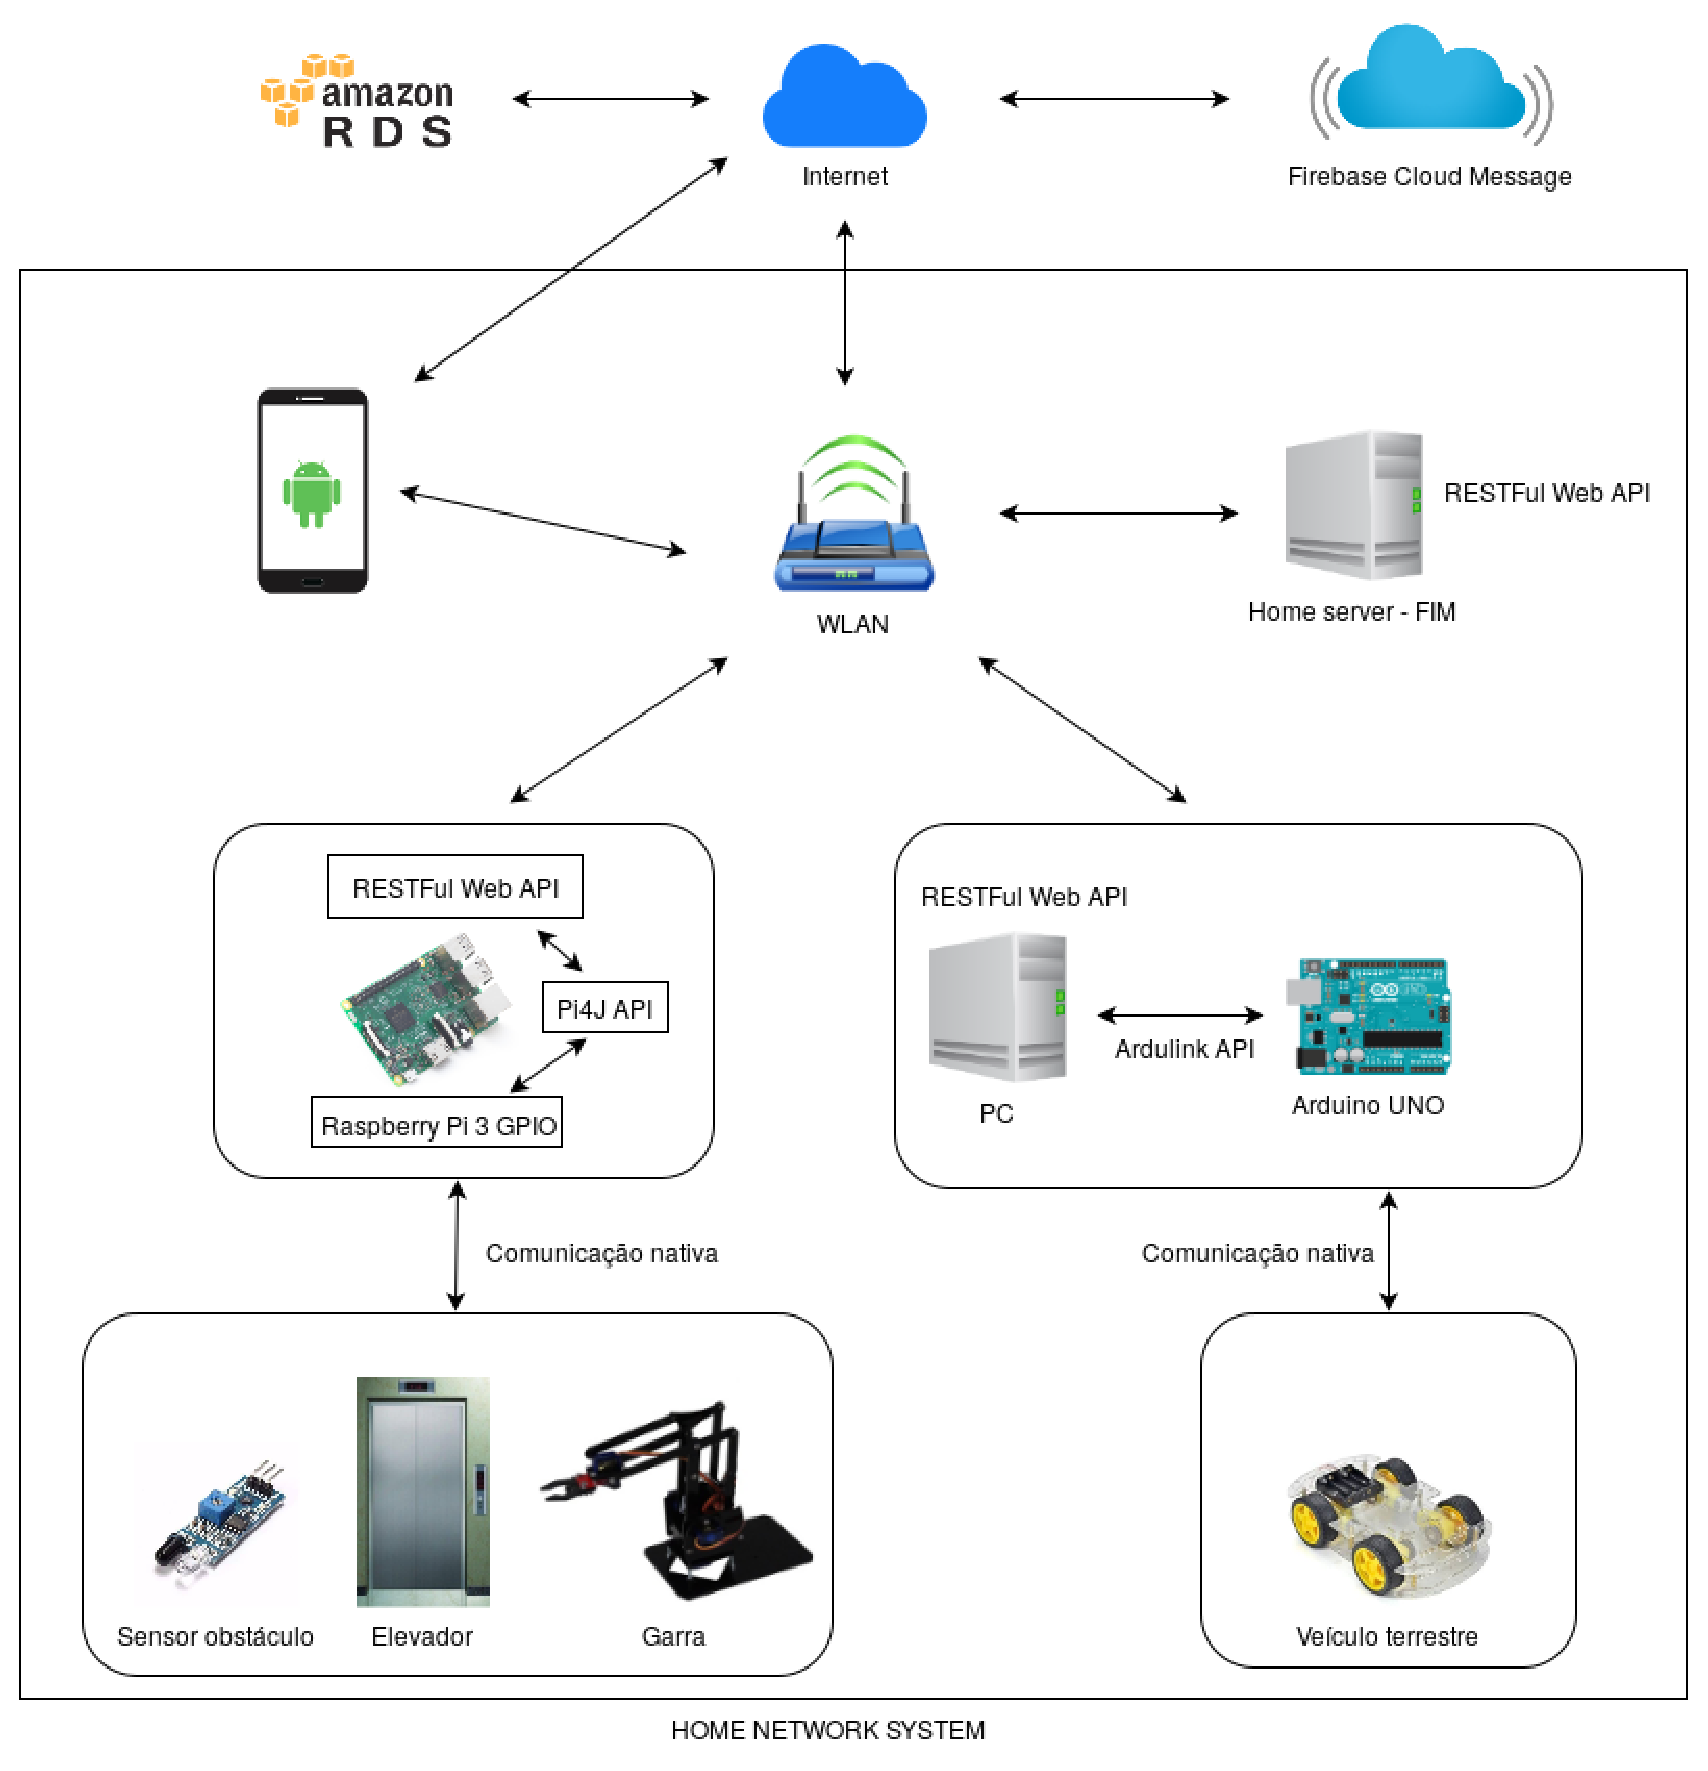
\includegraphics[width=1.0\columnwidth]{cenario} 
  \caption{Modelo do HNS utilizado neste trabalho.} 
  \label{fig:hnsworkmodel}
\end{figure}

\subsection{Levar compras}
\label{subsec:levarcompras}
O cenário ``Levar compras'' refere-se a funcionalidade (\textit{feature} ou característica)  oferecida pelo HS. Esta característica é provida através da composição dos serviços do elevador, veículo e garra. O cenário em questão pode ser visualizado na Figura \ref{fig:cenario} e é descrito a seguir.

\begin{enumerate}
\item Um usuário da casa (morador ou visitante), organiza as compras numa cesta (que tem formato expansível) e a coloca sobre o veículo terrestre.
\item O usuário então aciona o serviço ``Levar compras'' (disponibilizado pelo HS) através do seu \textit{smartphone}. O serviço então começa sua execução.
\item O FIM solicita informações de restrições do elevador e veículo terrestre, assim como quais objetos compõem a cesta. Este então verifica se a cesta colocada sobre o carro quebrou alguma restrição do mesmo e se a massa total dos objetos excedem a carga máxima do elevador.
\item Se nenhuma destas restrições foram quebradas o FIM solicita ao veículo terrestre que leve a as compras até as proximidades do elevador.
\item Assim que o veículo chega no seu destino, este envia uma mensagem ao FIM informando de sua chegada.
\item O FIM então requisita o elevador para levar as compras.
\item O elevador agora solicita a garra mecânica que pegue o cesto e coloque-o dentro do elevador.
\item Quando a garra completa a execução do seu serviço, esta avisa ao elevador.
\item Caso não haja nenhuma restrição, como por exemplo, alguma coisa que possa impedir a porta do elevador de fechar, então o elevador inicia o transporte das compras ao seu destino final e manda uma notificação ao HS.
\item HS Captura token referente ao \textit{smartphone} com Android\footnotemark \footnotetext{\url{https://www.android.com/intl/pt-BR_br/}} do usuário da casa.
\item Por fim, o HS solicita ao serviço de notificação \textit{Firebase Cloud Message}\footnotemark \footnotetext{\url{https://firebase.google.com/docs/cloud-messaging/?hl=pt-br}} que envie uma notificação para o usuário da casa, que a recebe no seu \textit{smartphone}. Assim completa-se a execução do serviço ``Levar compras''.
\end{enumerate}
        
\begin{figure}[!htb] \centering 
  \centering
  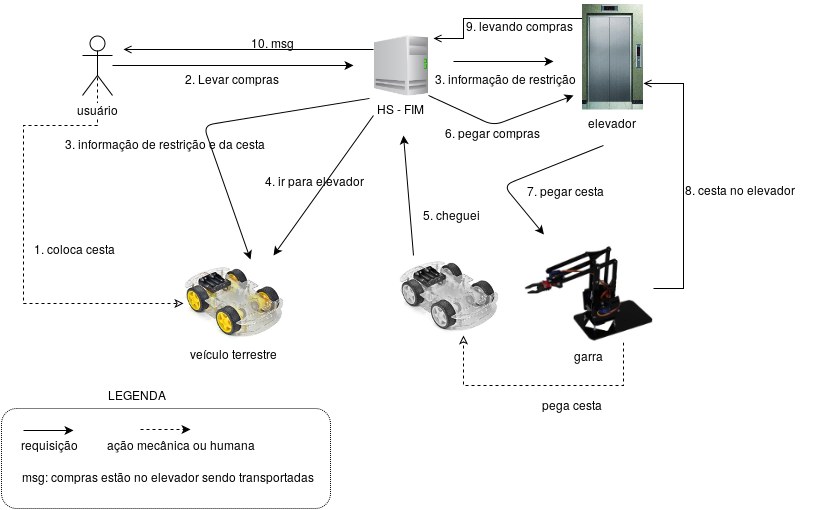
\includegraphics[width=1.0\columnwidth]{cenario_requests} 
  \caption{Cenário Levar compras.} 
  \label{fig:cenario}
\end{figure}

No cenário da Figura \ref{fig:cenario} o elevador não contém motores nem algum outro tipo de sistema elétrico ou mecânico, este é representado por uma caixa de papelão e um sensor de obstáculo acoplado. O veículo terrestre é representado por um programa carregado no Arduino UNO\footnotemark \footnotetext{\url{https://www.arduino.cc/en/Main/ArduinoBoardUno}}, o qual escuta através de sua porta serial mensagens provindas do PC (Figura \ref{fig:cenario}) e as processa simulando as funcionalidades ``Ir para elevador'' e ``cheguei''. Pela mesma porta serial o veículo terrestre encaminha suas mensagens ao PC. Os dispositivos veículo, elevador e garra podem ser visualizados na Figura \ref{fig:cenario_real}.

\begin{figure}[!htb] \centering 
  \centering
  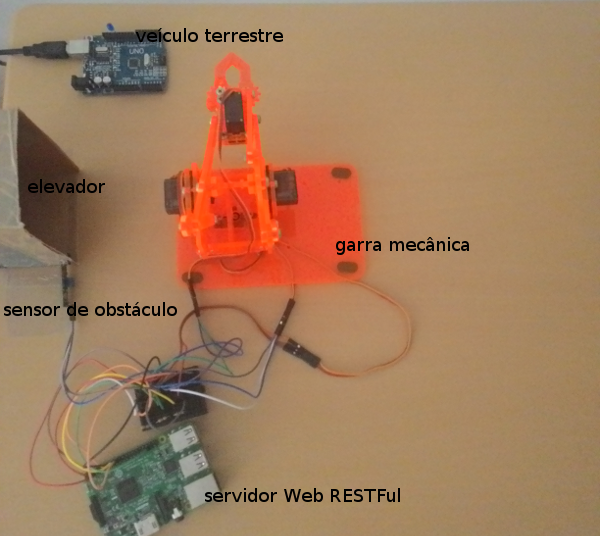
\includegraphics[width=0.8\columnwidth]{cenario_foto_real} 
  \caption{Dispositivos reais do cenário ``Levar compras''.} 
  \label{fig:cenario_real}
\end{figure}

\subsection{Execução do cenário}
De acordo com a Figura \ref{fig:cenario} o primeiro passo para inicializar a execução do cenário é colocar a cesta no veículo terrestre. Apesar do veículo ser simulado através de um software embarcado no Arduino, este necessita das informações dos objetos que se deseja transportar. Sendo assim, as informações da cesta são passadas quando o usuário executa o passo 2 (Levar compras). O usuário digita o ``id da cesta'' (no banco de dados) que se deseja transportar e clica em um botão para inicializar o serviço. Todas as cestas são compostas com miniaturas de objetos que normalmente são encontrados em supermercados, exemplos de cestas podem ser visualizados na Figura \ref{fig:exemplos_cesta}. Todos os objetos e cestas estão cadastradas no banco de dados na nuvem (amazon RDS\footnotemark \footnotetext{\url{https://aws.amazon.com/pt/rds/postgresql/}}), o qual foi apresentado na Figura \ref{fig:hnsworkmodel}. A lista de objetos que podem fazer parte de uma cesta é demonstrada na Figura \ref{fig:lista_objetos}, observe que para cada objeto é cadastrado suas características de massa, largura, comprimento, altura e diâmetro.

\begin{figure}[!htb] \centering 
  \centering
  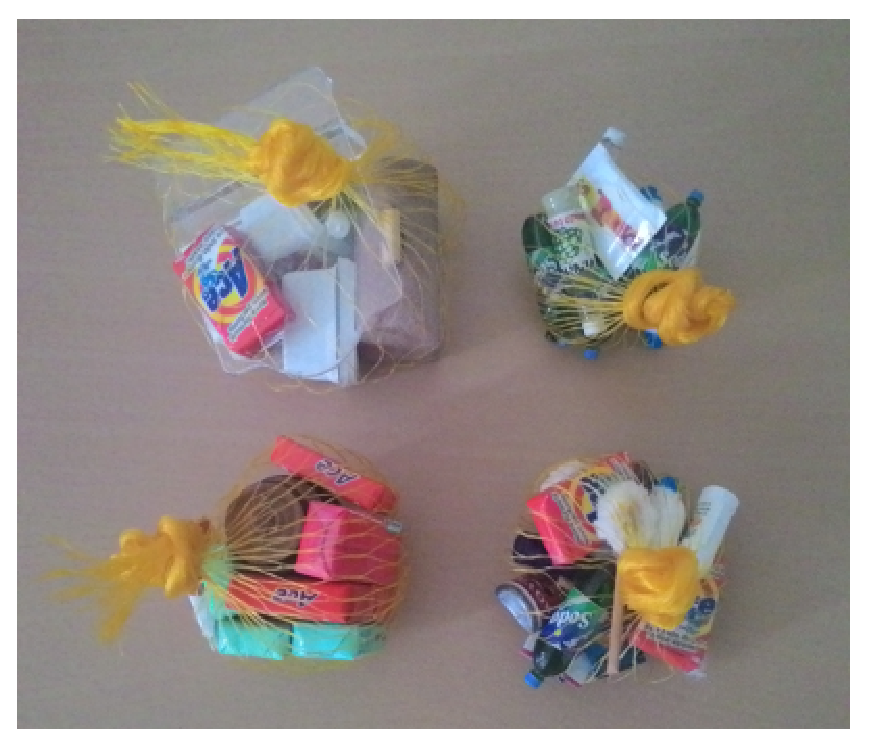
\includegraphics[width=0.8\columnwidth]{experimento/exemplos_cesta} 
  \caption{Exemplo de cestas do cenário ``Levar compras``.} 
  \label{fig:exemplos_cesta}
\end{figure}

\begin{figure}[!htb] \centering 
  \centering
  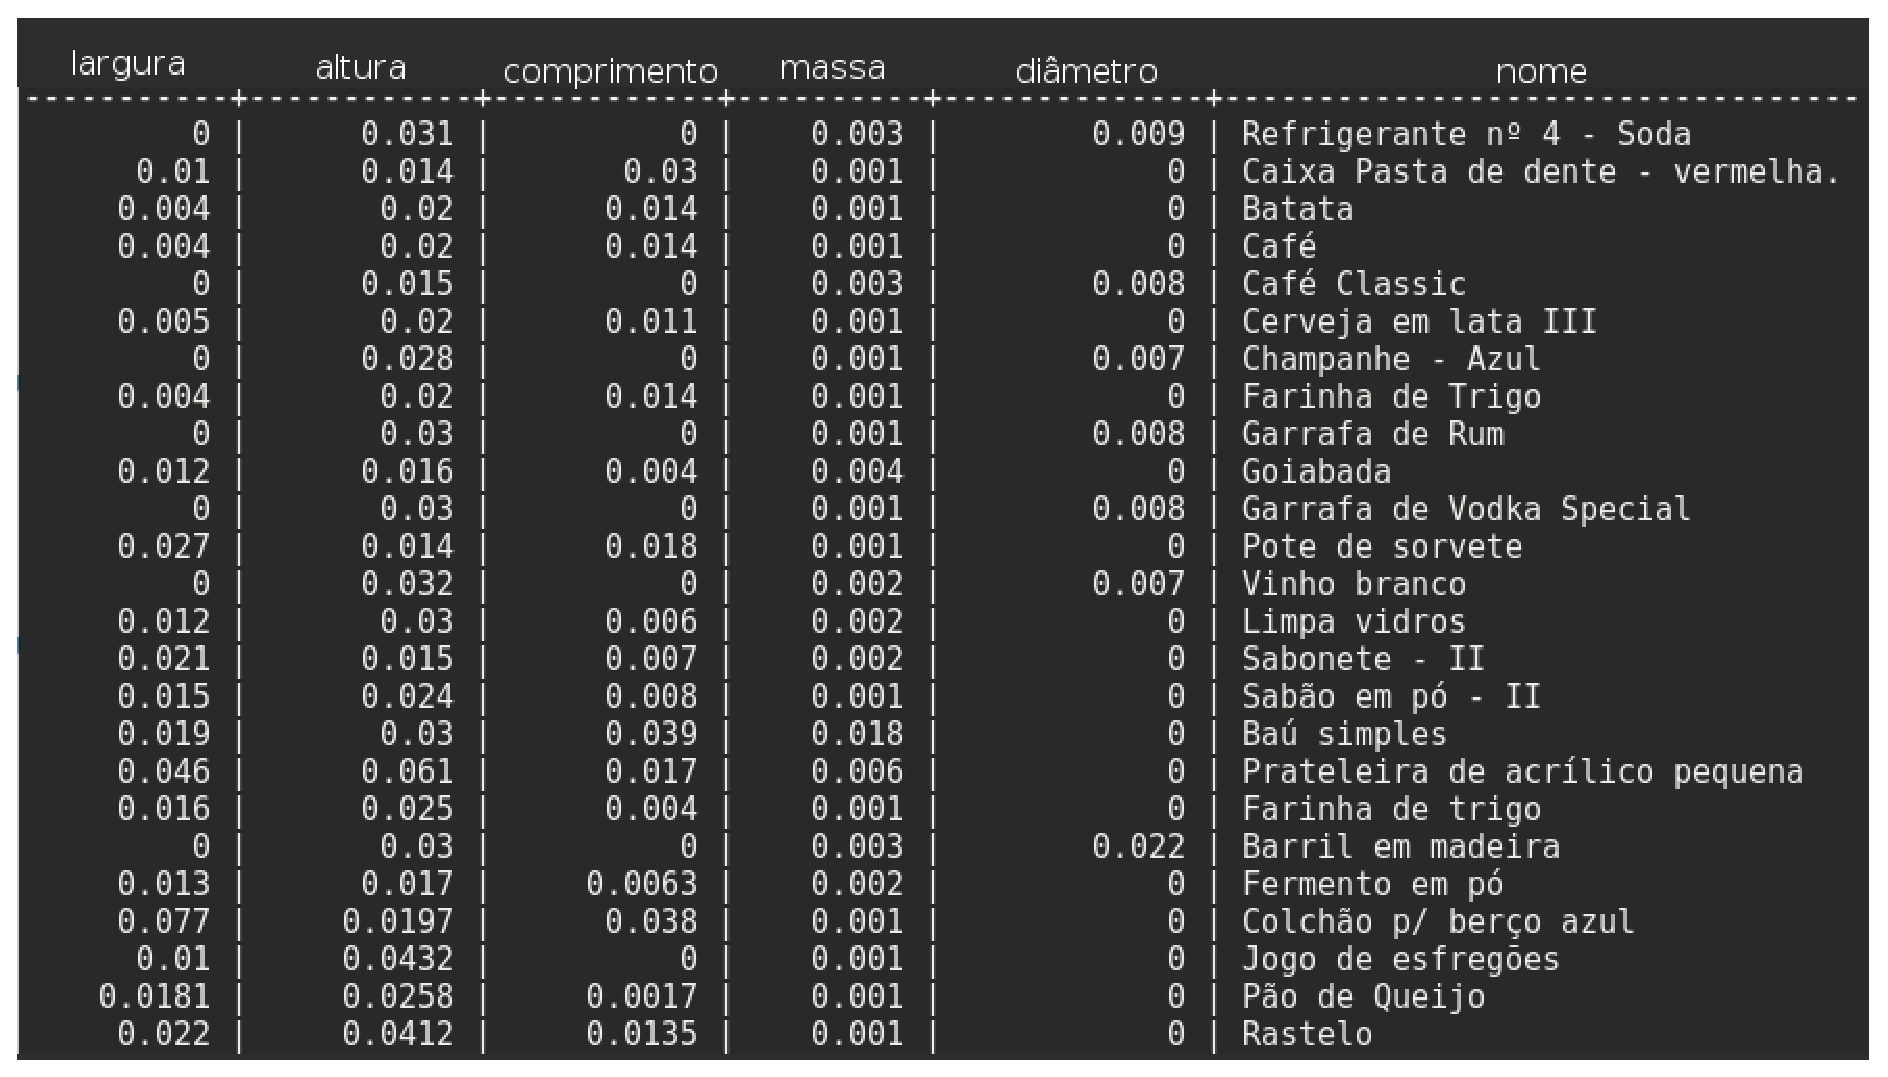
\includegraphics[width=0.8\columnwidth]{experimento/lista_items} 
  \caption{Lista dos objetos que podem ser utilizados para compor uma cesta.} 
  \label{fig:lista_objetos}
\end{figure}

Os próximos passos (3, 4, 5, e 6) do cenário podem ser executados sem mais problemas, pois já têm toda a informação necessária e não necessita de nenhuma intervenção humana. Isto já não acontece com o passo 7 (pegar cesta), pois este necessita de intervenção humana para a garra poder pegar a cesta e continuar a realizar o seu serviço, é preciso posicionar a cesta no lugar correto para a garra prender a cesta, como pode ser visto na Figura \ref{fig:garra_pegando_objeto}. Então, após a garra executar seu serviço esta manda uma mensagem para o elevador e, caso não tenha nada obstruindo a porta do elevador este inicia o transporte da cesta até o local desejado e manda uma mensagem para o fim. Daí em diante a execução do cenário continua da mesma forma com já explanado.

\begin{figure}[!htb] \centering 
  \centering
  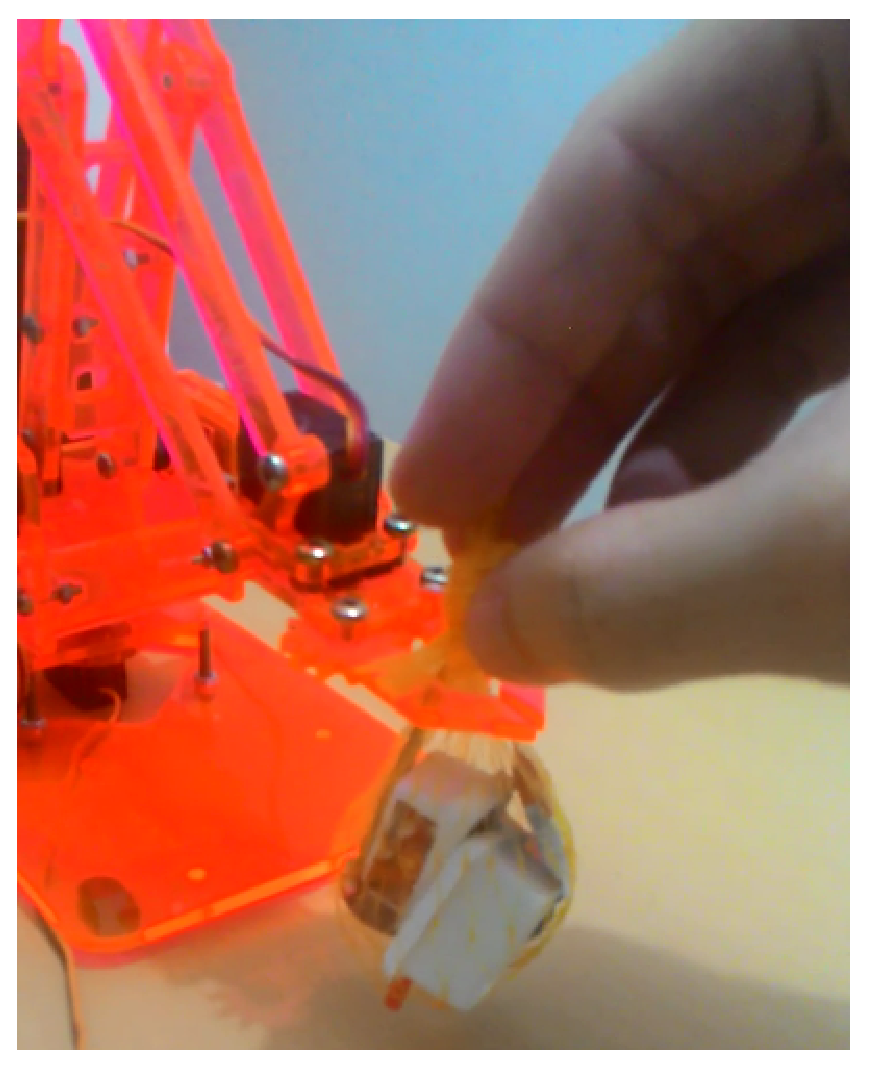
\includegraphics[width=0.8\columnwidth]{experimento/garra_pegando_objeto} 
  \caption{Cesta posicionada no local adequado por um humano, para que a garra possa prender a cesta adequadamente.} 
  \label{fig:garra_pegando_objeto}
\end{figure}

\subsection{Discussão da execução do cenário}
Para o cenário ``Levar compras`` foram confeccionadas e cadastradas no banco 66 cestas distintas. Antes de registrar as cestas no banco sempre era observado se a cesta cabia dentro do elevador quando colocadas de forma manual, e se também não ultrapassava os limites da porta, o limite de detecção do sensor de obstáculos. Então a cesta só era registrada caso coubesse no elevador e não estivesse em área que pudesse obstruir a porta. 

O cenário foi executado 66 vezes, uma para cada cesta, e pode-se observar que em algumas vezes o comportamento da garra provocava um efeito colateral indesejável (seção \ref{sec:featureinteraction}) na funcionalidade ``Levar carga'', pois a garra durante a execução do seu serviço (pegar cesta, mover de uma lado a outro , largar cesta) acabava por vezes não conseguindo que a cesta ficasse disposta dentro do elevador de uma maneira em que este pudesse continuar com o serviço de ``Levar carga'', apesar que para todos esses casos se esperava sempre como resultado o elevador levar as compras sem problemas, já que se era sabido que as cestas cabiam no elevador e, nenhuma delas feria as restrições de massa do carro nem do elevador. Tanto o veículo quanto o elevador sempre funcionaram de maneira esperada nestas execuções, pois o veículo sempre levava a carga para o local destinado avisando quando chegasse, e o elevador sempre acionava o serviço da garra, levava a carga  e avisava ao FIM quando não tinha obstáculo na porta, enquanto deixava de levar quando tinha, funcionando de maneira correta quanto as especificações de sua funcionalidade de locomoção, mas indo contra o comportamento esperado da funcionalidade pai ``Levar carga''. 

Concluindo as observações feitas até agora, o comportamento da garra junto com os tipos de objetos presentes na cesta faziam com que algumas vezes ocorressem locomoção destes durante o transporte da garra, e também no momento em que os objetos eram postos no compartimento do elevador. Nesse momento, os objetos as vezes geravam outras dimensões de cesta e/ou deslocamento da mesma, devido a natureza dos objetos e da forma como os objetos eram soltos pela garra. Sendo assim, para tentar detectar esses efeitos colaterais indesejáveis através de redes neurais, utilizou-se dos valores das grandezas físicas dos objetos (altura, massa, largura, comprimento, diâmetro) para gerar características que pudessem ser interessantes para a construção de modelos de redes neurais satisfatórios (ver seção \ref{sec:construmrn}).

Como todas as cestas estavam previamente cadastradas no banco de dados, a estas foram atribuídos valores de ``é efeito colateral'' ou ``não é efeito colateral'', a medida que se observava cada execução do cenário.

\section{Construção dos modelos de rede neural}
\label{sec:construmrn}
Os dados coletados na etapa de execução do cenário ``Levar carga'', 66 cestas, ainda estão muito brutos, observe que uma cesta deve conter pelo menos um objeto, como também pode conter muitos. Supomos que a cesta tenha 10 objetos, então o total de características da cesta seria $10.5=50$, pois cada objeto possui cinco características. Utilizar as características dos objetos desta forma, além de provavelmente não predizer nada em um modelo de rede neural, terá um custo computacional muito elevado. Para diminuir a quantidade de atributos e melhor qualificá-los gerou-se características a partir de todos os atributos dos objetos da cesta: média das alturas, dos comprimentos, das larguras, dos diâmetros e das massas, assim como o total de cada uma dessas medidas, e o total de itens. De ínicio então têm-se a seleção de 11 parâmetros.

Com a seleção prévia desses atributos, constriu-se um arquivo ``arff'', que é o tipo de arquivo padrão utilizado como \textit{dataset} pelo Weka\cite{Hall:2009}. Este \textit{dataset} é composto de 46 instâncias, cada uma com 11 atributos mais um que identifica a qual classe pertence. As outras 20 instâncias serão deixadas para um possível teste no cenário proposto, já com um classificador satisfatório, caso este seja possível de se construir.

O próximo passo utilizado nesse processo de seleção de atributos foi o de visualizar estes novos parâmetros par a par, e verificar quais pares parecem melhor separar as classes ``é efeito colateral'' ou ``não é efeito colateral''. Nas Figuras \ref{fig:plotall1}, \ref{fig:plotall2}, \ref{fig:plotall3} pode-se ter uma ideia de tal visualização. Dentre essas plotagens foram selecionadas duas plotagens (Figuras \ref{fig:tw_ad} e \ref{fig:tw_tm}), as quais parecem melhor separar as classes, são respectivamente os atributos ** e ** e, ** e **.

\begin{figure}[!htb] \centering 
  \centering
  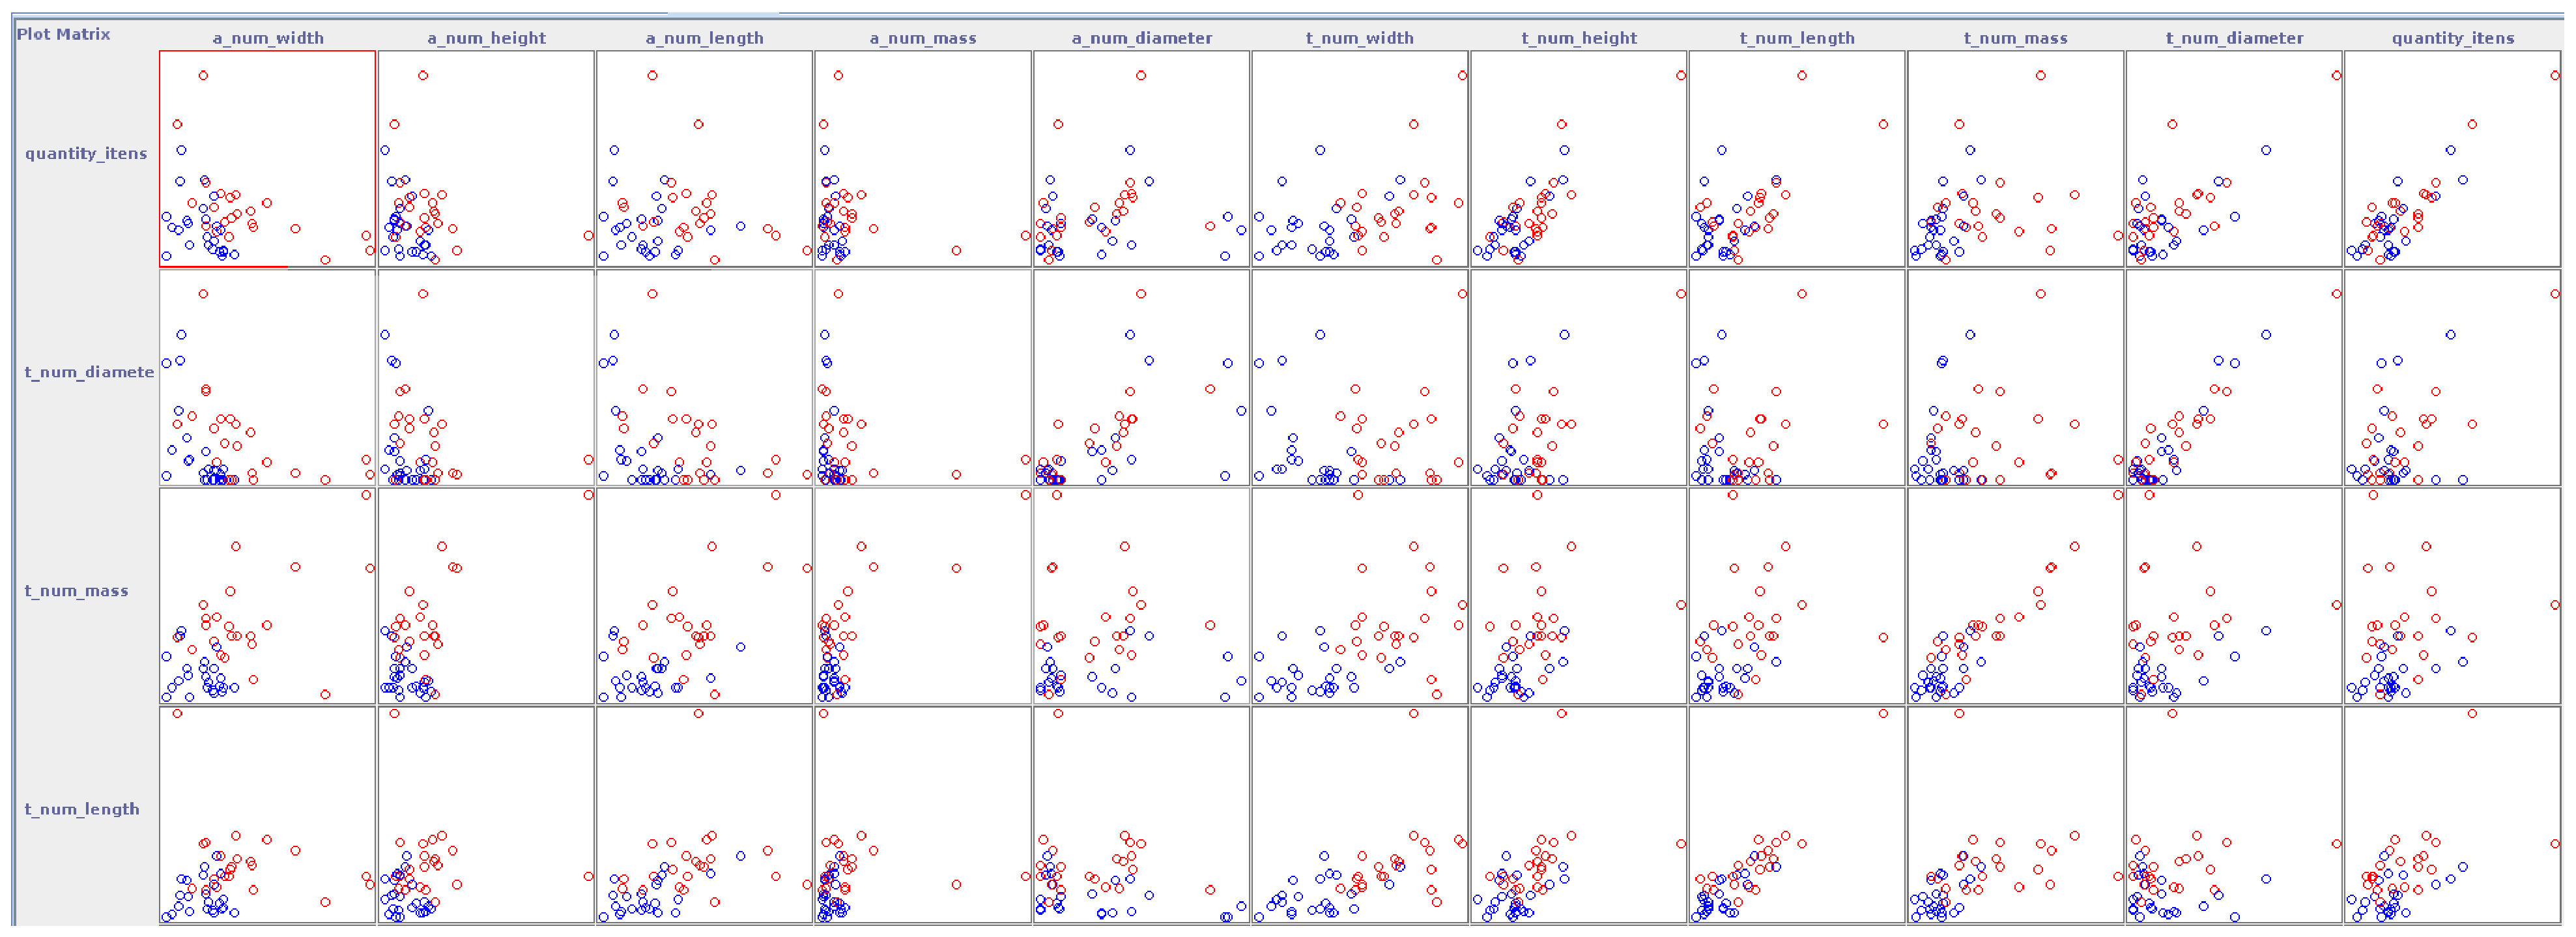
\includegraphics[width=1.0\columnwidth]{experimento/all1_plot} 
  \caption{Plotagem 1 de todas a médias e totais das características dos objetos, conjugadas par a par.} 
  \label{fig:plotall1}
\end{figure}

\begin{figure}[!htb] \centering 
  \centering
  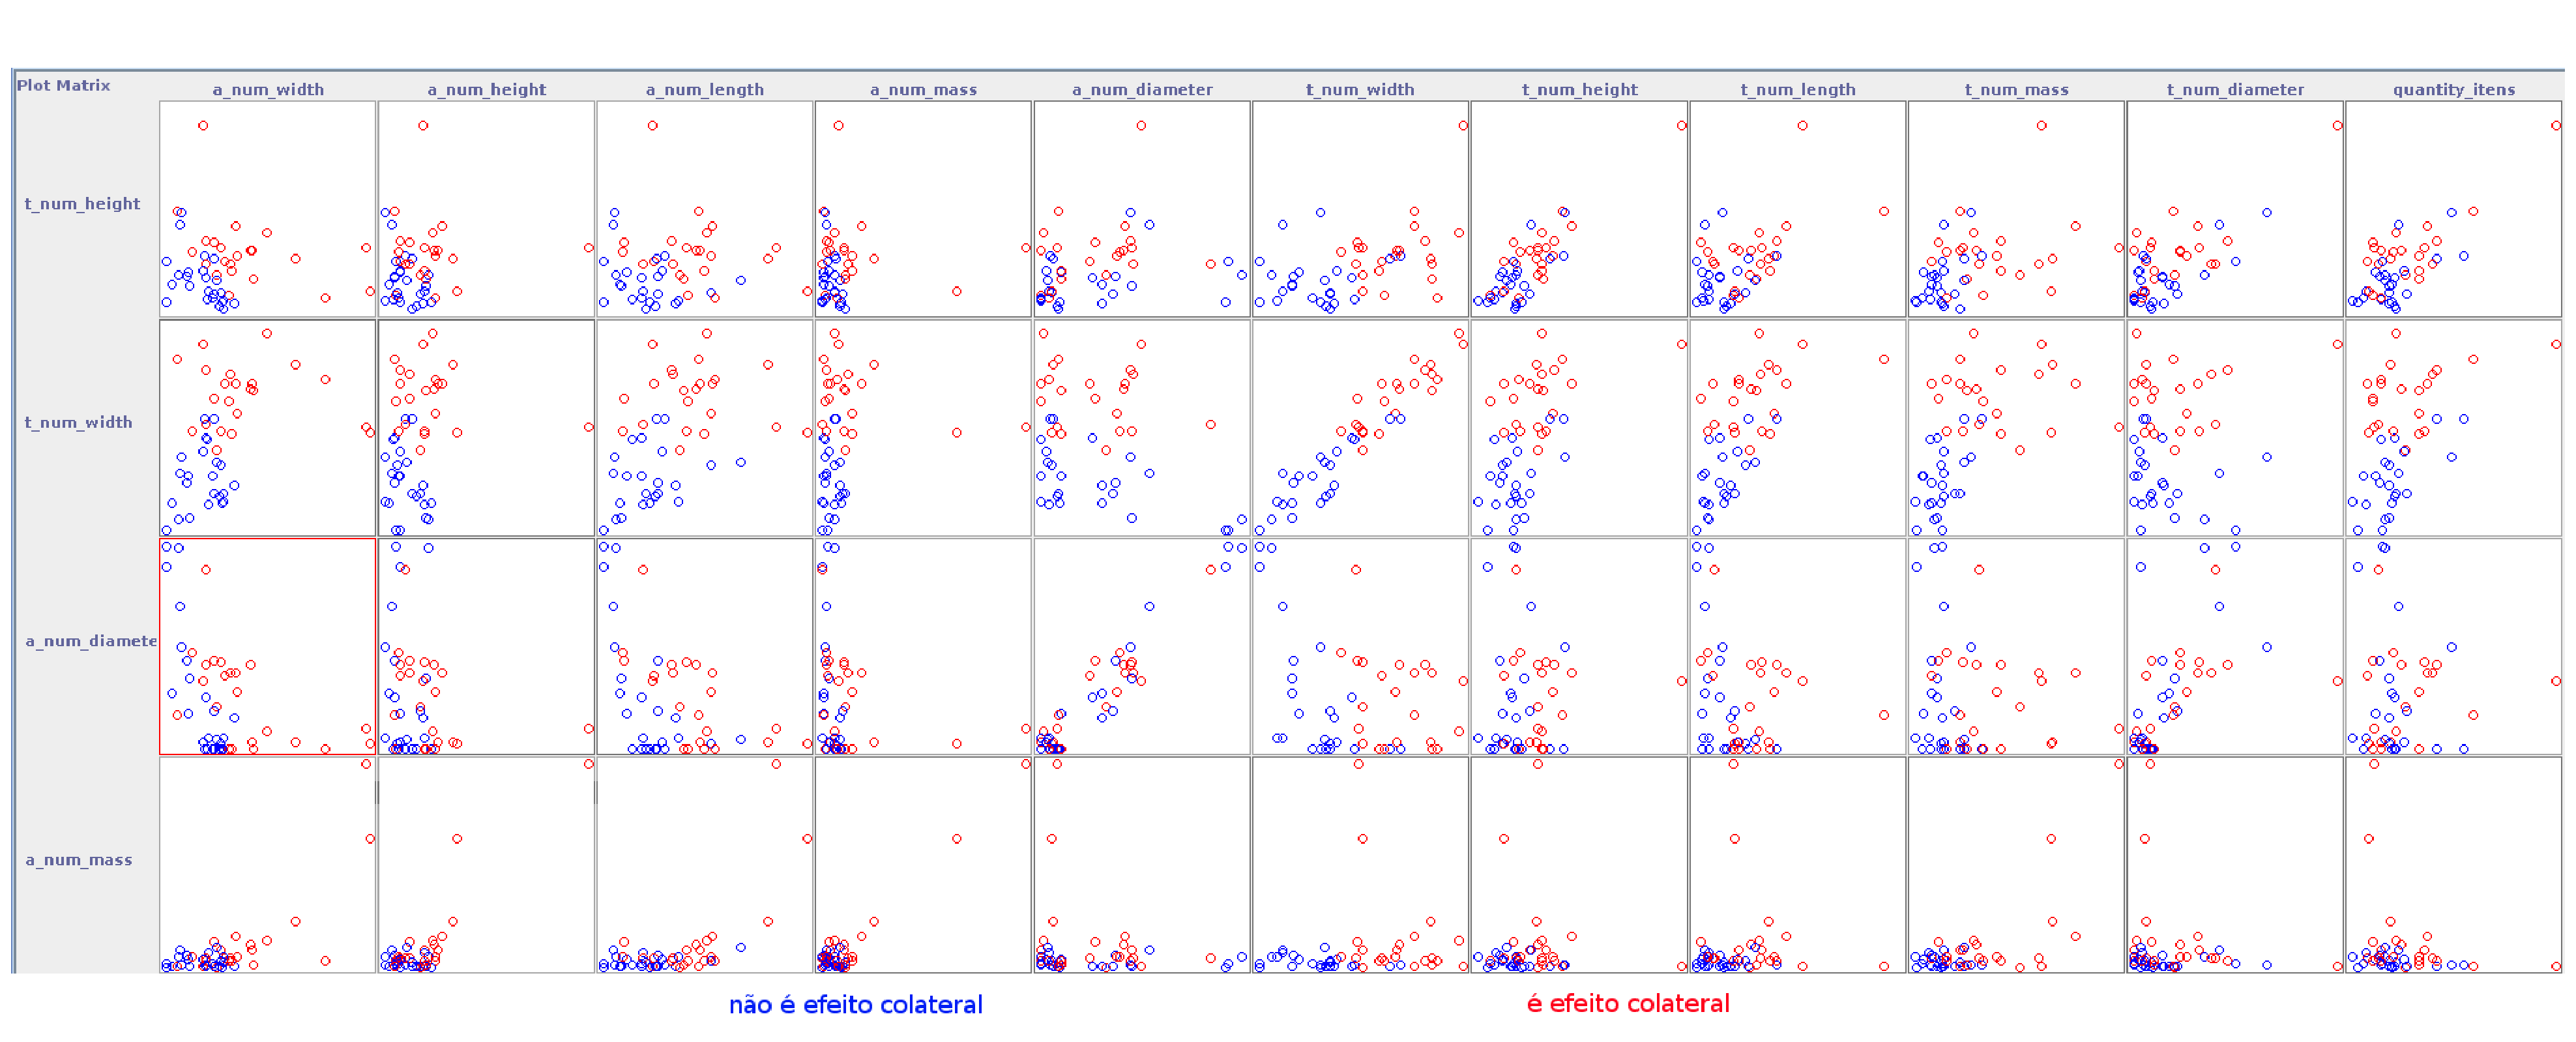
\includegraphics[width=1.0\columnwidth]{experimento/all2_plot} 
  \caption{Plotagem 2 de todas a médias e totais das características dos objetos, conjugadas par a par.} 
  \label{fig:plotall2}
\end{figure}

\begin{figure}[!htb] \centering 
  \centering
  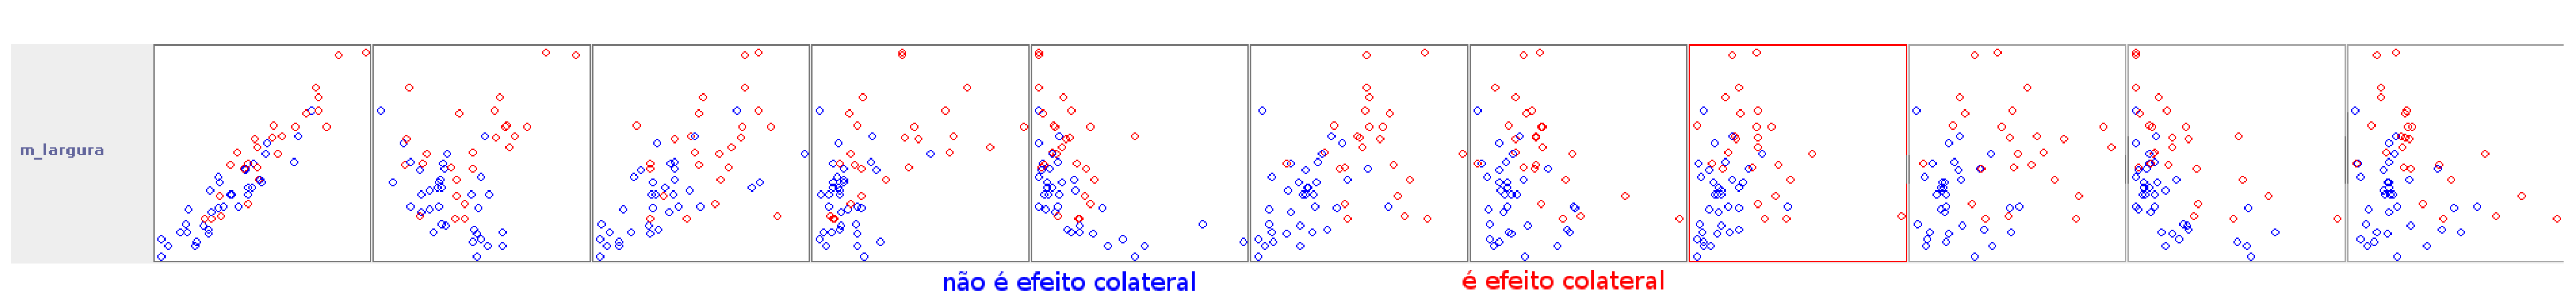
\includegraphics[width=1.0\columnwidth]{experimento/all3_plot} 
  \caption{Plotagem 3 de todas a médias e totais das características dos objetos, conjugadas par a par.} 
  \label{fig:plotall3}
\end{figure}

\begin{figure}[!htb] \centering 
  \centering
  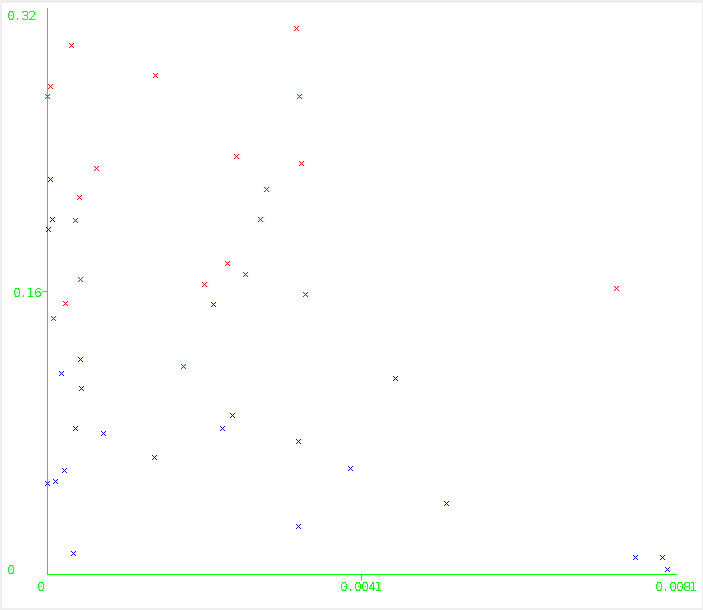
\includegraphics[width=0.8\columnwidth]{experimento/tw_ad} 
  \caption{Plotagem dos atributos... } 
  \label{fig:tw_ad}
\end{figure}
\begin{figure}[!htb] \centering 
  \centering
  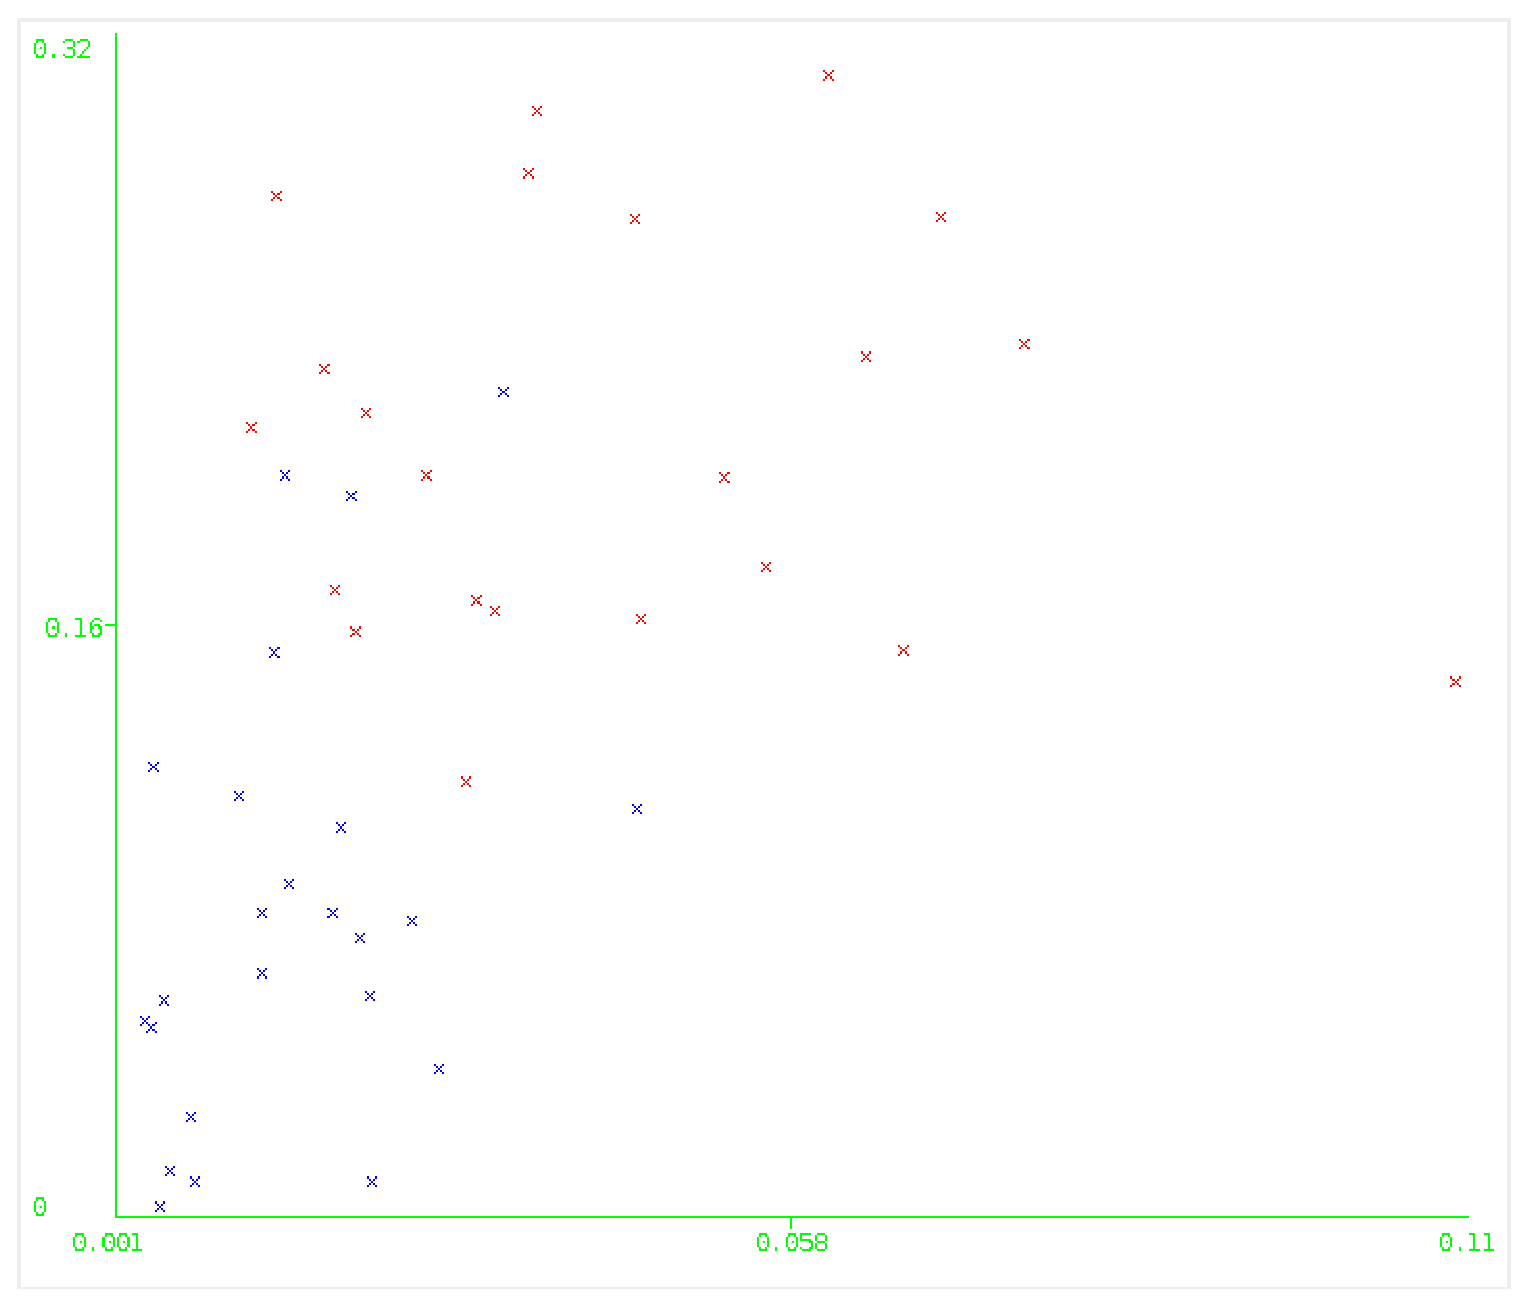
\includegraphics[width=0.8\columnwidth]{experimento/tw_tm} 
  \caption{Plotagem dos atributos... } 
  \label{fig:tw_tm}
\end{figure}

Procedimentos utilizados - experimento:
-gera uma plotMatriz dos dados do dataset
-verifica quais dados poderiam ser melhor separados por uma curva(par a par)

-neste caso, visualmente são esse abaixo:
t_num_width e t_num_diameter
(quem não tem width, tem diameter e vice e versa)
t_num_mass e t_num_width

-testa com alguma combinação distinta dos parâmetros acima
t_num_width, t_num_mass, t_num_diameter 

\section{Metodologia para validação dos modelos}

**ver se dar tempo de gerar curva roc(verifdicar o motivo da roc, é viavel para este cenário) e precision e recall dos resultados dos 3 modelos**

MOTIVO:
escolher os melhores parametros para o modelo em questão, neste caso, rede neural.

 machine learning and statistics, feature selection, also known as variable selection, attribute selection or variable subset selection, is the process of selecting a subset of relevant features (variables, predictors) for use in model construction. Feature selection techniques are used for three reasons:

        simplification of models to make them easier to interpret by researchers/users,[1]
        shorter training times,
        enhanced generalization by reducing overfitting[2](formally, reduction of variance[1])

The limitation to just one layer of hidden neurons is justified by the fact that one hidden layer is enough to approximate any continuous function (6,7).\cite{Pasini:2015}

-Verifica a generalização utilizando técnicas estaitisticas, tais como, stratifyed-k-crossvalidation e/ou randomized-holdout

-escolhe o melhor modelo baseado no que você quer do modelo, neste caso o que tiver melhor recall, seguido de accuracy. POIS É MELHOR ERRAR DIZENDO QUE É, DO QUE ERRAR DIZENDO QUE NÃO É.

-gera um classificador com todo o dataset verificado na etapa anterior.
-testa esse classificador com um dataset distinto do anterior.
-DEMONSTRA OS RESULTADOS E COMPARA COM OS TESTES ANTERIORES.

\section{Resultados}
-modelo de clasificado bom para o cenário
-implantar o classificador no sistema
Para verificar a vericidade da hipótese...


\xchapter{Conclusão}{Síntese da investigação e dos experimentos realizados nesta monografia}
\label{ch:conclusion}

Solutions for specific feature interactions can then be generalized to other interactions of the same category.

%\xchapter{Trabalhos Futuros}{Possíveis explorações adicionais que derivam deste trabalho}
%
%\input{trabalhos_futuros}

%% Parte pos-textual
\backmatter

% Apendices
% Comente se naoo houver apendices
\appendix

% Eh aconselhavel criar cada apendice em um arquivo separado, digamos
% "apendice1.tex", "apendice.tex", ... "apendiceM.tex" e depois
% inclui--los com:
% \include{apendice1}
% \include{apendice2}
% ...
% \include{apendiceM}

% Bibliografia
% É aconselhável utilizar o BibTeX a partir de um arquivo, digamos "biblio.bib".
% Para ajuda na criação do arquivo .bib e utilização do BibTeX, recorra ao
% BibTeXpress em www.cin.ufpe.br/~paguso/bibtexpress
\bibliographystyle{abntex2-alf}
\bibliography{biblio}

%% Fim do documento
\end{document}
%------------------------------------------------------------------------------------------%
